%%%%%%%%%%%%%%%%%%%%%%% file template.tex %%%%%%%%%%%%%%%%%%%%%%%%%
%
% This is a template file for The European Physical Journal PLUS
%
% Copy it to a new file with a new name and use it as the basis
% for your article
%
%%%%%%%%%%%%%%%%%%%%%%%% Springer-Verlag / Societa` Italiana di Fisica  %%%%%%%%%%%%%%%%%%%%%%%%%
%
%\begin{filecontents}{leer.eps}
%!PS-Adobe-2.0 EPSF-2.0
%%%CreationDate: Mon Jul 13 16:51:17 1992
%%%DocumentFonts: (atend)
%%%Pages: 0 1
%%%BoundingBox: 72 31 601 342
%%%EndComments
%
%gsave
%72 31 moveto
%72 342 lineto
%601 342 lineto
%601 31 lineto
%72 31 lineto
%showpage
%grestore
%%%Trailer
%%%DocumentFonts: Helvetica
%\end{filecontents}
%
\documentclass[epj]{svjour}
% Remove option referee for final version
%
% Remove any % below to load the required packages
%\usepackage{latexsym}
\usepackage{mathtools} % Loads amsmath
\usepackage{graphics}
\usepackage{amsmath}
\usepackage{amssymb}
\usepackage{latexsym}
\usepackage{amsfonts}
\usepackage{authblk}
\usepackage{xfrac}
\usepackage{graphicx}
%\usepackage[colorlinks=true,linkcolor=black, citecolor=blue, urlcolor=blue]{hyperref} % for hyperrefs
%\usepackage{cleveref}
%\usepackage[authoryear]{natbib}
\usepackage{gensymb}  % provides macro \degree which works in text and math
\usepackage{color}
%\usepackage{enumitem} 
\usepackage{bm}
\usepackage{multirow}
\usepackage{cite}
\usepackage{subcaption} % For subfigure
\captionsetup{compatibility=false}
\usepackage{wrapfig}
%\usepackage{caption} % Caption in subfigure
\usepackage{tikz}
\usetikzlibrary{arrows}

% for quotes
\usepackage [english]{babel}
\usepackage [autostyle, english = american]{csquotes}
\MakeOuterQuote{"}

% for flow charts
% Define block styles

\usetikzlibrary{patterns}
\usetikzlibrary{shapes,arrows}
\tikzstyle{discre} = [rectangle, draw, fill=white!20, 
text width=6em, text centered, minimum height=3em, node distance=3.5cm, line width=1pt]
\tikzstyle{decision} = [diamond, draw, fill=white!20, 
text width=3em, text badly centered, node distance=2cm, inner sep=1pt, line width=1pt]
\tikzstyle{block} = [rectangle, draw, fill=white!20, 
text width=6em, text centered, minimum height=3em, node distance=3.5cm, line width=1pt]
\tikzstyle{blockEq} = [rectangle, draw, fill=white!20, 
text width=8em, text centered, minimum height=3em, node distance=3.5cm, line width=0pt]
\tikzstyle{cloud} = [draw, ellipse,fill=white!20, node distance=4cm,
text centered, text width=3em, minimum height=2em, line width=1pt]
\tikzstyle{line} = [draw, -{latex'}, line width=1.0pt]

% For merging cells 
\usepackage{array}
\usepackage{booktabs}
\setlength{\heavyrulewidth}{1.5pt}
\setlength{\abovetopsep}{4pt}

% etc
%

\newcommand{\eq}[1]{Eq.~(\ref{#1})}
\newcommand{\eqnolabel}[1]{(\ref{#1})}
\newcommand{\eqs}[1]{Eqs.~(\ref{#1})}
\newcommand{\eqsthru}[2]{Eqs.~(\ref{#1})--(\ref{#2})}
\newcommand{\eqsand}[2]{Eqs.~(\ref{#1}) and (\ref{#2})}
\newcommand{\tbl}[1]{Table~\ref{#1}}
\newcommand{\tblnolabel}[1]{\ref{#1}}
\newcommand{\tbls}[1]{Tables~\ref{#1}}
\newcommand{\tblsthru}[2]{Tables~\ref{#1}--\ref{#2}}
\newcommand{\tblsand}[2]{Tables~\ref{#1} and \ref{#2}}
\newcommand{\fig}[1]{Fig.~\ref{#1}}
\newcommand{\fignolabel}[1]{\ref{#1}}
\newcommand{\figs}[1]{Figs.~\ref{#1}}
\newcommand{\figsthru}[2]{Figs.~\ref{#1}--\ref{#2}}
\newcommand{\figsand}[2]{Figs.~\ref{#1} and \ref{#2}}
\newcommand{\sxn}[1]{Section~\ref{#1}}

\newcommand{\revised}[1]{{\color{red}{#1}}}
\newcommand{\tsup}[1]{\textsuperscript{#1}}
\newcommand{\tsub}[1]{\textsubscript{#1}}

\newcommand{\erez}[1]{{\color{blue}{\textsuperscript{EREZ:}#1}}}
\newcommand{\roy}[1]{{\color{blue}{\textsuperscript{ROY:}#1}}}

\newcommand{\keff}{{\ensuremath{k_{\textrm{\scriptsize{eff}}}}}}
\newcommand{\beff}{\ensuremath{\beta_{\textrm{eff}}}}
\newcommand{\rr}{\ensuremath{\bm{r}}}
\newcommand{\OO}{\ensuremath{\hat{\bm{\Omega}}}}
\newcommand{\bnabla}{\ensuremath{\bm{\nabla}}}
\newcommand{\rE}{\ensuremath{(\rr,E)}}

\newcommand{\ftr}{\ensuremath{\phi_{\textrm{\scriptsize{tr}}}}}
\newcommand{\jtr}{\ensuremath{\bm{J}_{\textrm{\scriptsize{tr}}}}}
\newcommand{\jtrr}{\ensuremath{J_{\textrm{\scriptsize{tr}}}}}
%\newcommand{\mcL}{\mathcal{L}}
\newcommand{\mcL}{\tau}
\newcommand{\pl}[1]{\ensuremath{P_l(#1)}}
\newcommand{\dx}{\ensuremath{\Delta x}}

%
\graphicspath{ {./figures/} }
% ---------------------------------------------------
\begin{document}
%
\title{High-accuracy neutron diffusion calculations based on integral transport theory}
%\subtitle{}
\author{
	Roy Gross\inst{1} \and 
	Daniele Tomatis\inst{2} \and 
	Erez Gilad\inst{1}\thanks{\email{gilade@bgu.ac.il} (corresponding author)}
}                     % Do not remove
%
%\offprints{}          % Insert a name or remove this line
%
\institute{
	The Unit of Nuclear Engineering, Ben-Gurion University of the Negev, 8410501 Beer-Sheva, Israel 
	\and
	CEA, DEN, Service d'{\'e}tudes des r\'eacteurs et de math\'ematiques appliqu\'ees (SERMA),
	Universit\'e Paris-Saclay, F-91191 Gif-sur-Yvette, France}
%
\authorrunning{Gross, Tomatis \& Gilad} 
\titlerunning{Integral transport correction to diffusion calculations}
\date{Received: date / Revised version: date}
% The correct dates will be entered by Springer
%
\abstract{
In this paper, the Ronen method is developed, implemented, and applied to resolve the neutron flux and the criticality eigenvalue in one-dimensional simple homogeneous problem and in more complex heterogeneous benchmarks. The Ronen method is based on iterative calculations of the multigroup diffusion correction factors using a multigroup diffusion model and is driven by the solutions of the integral transport equation. The spatially-dependent diffusion constants are modified locally in order to produce new estimates of the surface currents using an integral transport expression. The diffusion solver employed in this study uses finite differences and the transport-corrected currents are introduced into the numerical scheme using drift terms. The corrected solutions are compared against reference results obtained by a discrete ordinate code. Boundary conditions are discussed and proper approximations are introduced to conserve the particle balance. The results match well with the reference solutions, especially in the limit of fine meshes, but slow convergence of the scalar flux is reported.
% 
\PACS{
	{28.00.00}{Nuclear engineering and nuclear power studies} \and
	{28.20.Gd}{Neutron transport: diffusion and moderation} \and
	{05.60.-k}{Transport processes} \and
	{28.41.-i}{Fission reactors}
     } % end of PACS codes
  \keywords{
  	neutron diffusion -- integral transport -- non-linear transport correction
  }
} %end of abstract
%
\maketitle
%
% ---------------------------------------------------
\section{Introduction}
\label{sec:intro}

Neutron transport calculations on a full core scale can be a highly intensive computational task. High-fidelity core design optimization or transient analyses can quickly become computationally impractical when using transport methods~\cite{Kim-2019}. For example, to achieve a 1\% accuracy in the local flux/power estimation, an order of 10\tsup{11} histories is needed in a full-core Monte Carlo calculation~\cite{Martin-2012}. Another problem is the huge number of variables and parameters to be stored and used during computation, e.g., tallies, geometry, cross sections, and depletion data. A conservative estimation of the memory needed for reasonably accurate full-core Monte Carlo neutronic calculation is in the range of terabytes (TBs)~\cite{Martin-2012}. The growing demand for high-accuracy and high-precision full-core computations challenges not only today’s high-end computing systems but will also challenge the near future (e.g., Exascale) computers~\cite{Martin-2012,Smith-2011,Kim-2019}.  

To overcome this difficulty, faster (and less accurate) multigroup neutron diffusion solvers are frequently used~\cite{Lawrence-1986,Smith-1986}. However, future Gen-IV reactor designs are characterized by strong heterogeneity in the core, e.g., axial and radial seed-blanket structures, as in the French ASTRID SFR CVF design~\cite{Bertrand-2016}, challenging the accuracy of diffusion calculations. Moreover, modern calculation schemes evolve towards so-called "best-estimate" codes, aiming at high accuracy~\cite{IAEA-BE-2008}. 

A crucial issue in obtaining an accurate diffusion calculation is the formulation of the diffusion coefficient~\cite{Bell-1970,Pounders-2009}. The calculation of this parameter should be based on physical insights from the transport equation such that the resulting improved ("transport corrected") diffusion approximation can capture the transport phenomena of interest. Such transport corrections can be divided into two main classes. The first class is based on extending the $P_1$ model equations (and the associated boundary conditions) along with some closure scheme, such as the well-known $SP_3$ approximation~\cite{Brantley-2000}. The second class, to which this study belongs, is based on the re-calculation of the diffusion correction factors within the multigroup diffusion framework~\cite{Tomatis-2011}. 

In this paper, the development, implementation, and qualification of the Ronen Method~\cite{Ronen-2004} in one-dimensional homogeneous and heterogeneous plane geometry is reported. This method is implemented as a highly accurate multigroup neutron diffusion solver based on novel transport corrections. The main hypothesis underlying the Ronen method is based on iterative calculations of the multigroup diffusion coefficients driven by the solutions of the integral transport equation~\cite{Ronen-2004,Tomatis-2011}. 

%This study addresses a critical issue in contemporary nuclear reactor calculations, which constitutes an inherent difficulty that will not be solved in the near future merely by increased computational capabilities. As modern and advanced nuclear systems become more complex and heterogeneous, the requirements for more precise and accurate calculations increase as well~\cite{Smith-2011,Martin-2012,Smith-2013,Tomatis-2011,Kim-2019}. This trend is not likely to fade away. In light of this trend, the development of highly accurate neutron diffusion calculations is of great importance for nuclear reactor's operation, safety, research, and design purposes.

The theoretical background is detailed in~\sxn{sec:theory}, the numerical implementation is described in~\sxn{sec:imp}, the results are presented in~\sxn{sec:res}, and conclusions are brought in~\sxn{sec:conc}.

%
% ---------------------------------------------------
\section{Theoretical background}
\label{sec:theory}

%
% ---------------------------------------------------
\subsection{The Ronen method}
\label{sec:RM}

In 2004, Ronen~\cite{Ronen-2004} suggested to derive corrected diffusion coefficients using Fick's law and more accurate estimations of the neutron currents by means of integral transport operators, whereas the neutron flux is resolved by diffusion theory. Denoting the integral transport and diffusion currents by $\jtr\rE$ and $\bm{J}_D\rE$, respectively, the Ronen idea is based on changing the diffusion coefficient such that
\begin{equation}\label{eq:Fick}
\bm{J}_D\rE = -D\rE\bnabla\phi\rE = \jtr\rE \,\, . 
\end{equation}

Since these accurate estimates of the currents are based on a known flux distribution, it was also suggested to execute new diffusion calculations, thus updating iteratively the diffusion coefficients in the global calculation. 
\begin{equation}\label{eq:RM-it}
D^{(k+1)}\rE = -\frac{\lvert\jtr^{(k)}\rE\rvert}{\lvert\bnabla\phi^{(k)}\rE\rvert} \,\, ,
\end{equation}
where $k$ is the iteration index. The use of a tensor notation is needed for the diffusion coefficient in general multidimensional problems.

The motivation for this method was to overcome the inherent limitation of Fick's law requiring smooth flux gradients and thus small neutron absorption rate with respect to scattering in general. Nevertheless, isotropic scattering remained as a basic postulate.
For example, in a homogeneous slab with void boundary conditions, Eq.~\eqref{eq:RM-it} takes the following form~\cite{Ronen-2004} 
\begin{equation}\label{eq:RM-it-1D-slab}
D^{(k+1)}(x,E) = -\frac{\frac{1}{2}\int_0^a dx' E_2[\sigma(E)\lvert
	x-x'\rvert]\text{sign}(x-x')q^{(k)}(x',E)}
{\partial \phi^{(k)}(x,E)/\partial x} \,\, .
\end{equation}

This idea was later used by Tomatis and Dall'Osso~\cite{Tomatis-2011}, who provided a numerical demonstration in a simple slab problem. Instead of updating the diffusion coefficient by the ratio of the current and the flux gradient, as in Fick's law, they adopted the Coarse Mesh Finite Differences method (CMFD) for taking into account the new currents estimated by the integral transport operator in the diffusion solver. 
%
%They proposed to update non-linearly the diffusion coefficients at the cell interfaces of the spatial mesh by the coarse mesh finite differences method (CMFD).
%
This technique, largely adopted in the literature of nodal methods~\cite{Smith-1983,Lawrence-1986}, can avoid indeterminate divisions in case of vanishing flux gradients. They tested this implementation in a homogeneous bare slab using two-group cross sections representative of a realistic PWR assembly. It was observed that the Ronen method (RM) could drive the flux distribution away from diffusion and closer to the reference solution of the integral Boltzmann transport equation, regardless of the initial formulation used for the diffusion coefficient. As expected, the largest errors were located near the boundary, where the transport effects are most pronounced, slowly decreasing even after many iterations.% Their work was limited to the homogeneous slab, and resolved neutron diffusion on the same discretized spatial mesh used for the reference from neutron transport.

%
% ---------------------------------------------------
\subsection{The one-dimensional Peierls equation}
\label{sec:Peierls}

There are several ways to drive the integral expression for the flux in slab geometry. Most of them start with assuming homogeneous and isotropic scattering and sources, yielding the \emph{Peierls equation} \cite{Davison-1957,Case-1967,Bell-1970,Pomraning-1973,Duderstadt-1979,Lewis-1984}. The derivation of expression for slab geometry (of thickness $a$) is straightforward, yielding
\begin{eqnarray}\label{eq:flux-slab-l-0-no-bndry-terms}
\phi(x,E)&=&\frac{1}{2}\int_0^a { dx'
	E_1\left[\sigma(E)\lvert x-x'\rvert\right] q(x',E) 
}\nonumber \\
&=& \frac{1}{2}\int_0^a { \!\!\! dx'
	E_1\left[\sigma(E)\lvert x-x'\rvert\right]
	\left[
	\int_0^\infty { \!\!\! dE'
		\sigma_s(E\leftarrow E')\phi(x',E') 
	} + S(x',E)
	\right] 
} \,\, ,
\end{eqnarray}

where $E_1(x)$ is a first order exponential integral~\cite{Abramowitz-1964}. Note that this expression does not include the contribution of uncollided neutrons originated from an incoming angular flux at the boundaries.

Another starting point for the derivation of the integral expression for the flux in slab geometry is to directly integrate along a line the transport equation~\cite{Davison-1957,Pomraning-1973,Duderstadt-1979,Lewis-1984}
\begin{eqnarray}\label{eq:full-ITE-w-bndry-terms}
\psi(\rr,\OO) &=& \int_0^R { dR'
	q(\rr-R'\OO,\OO) e^{-\mcL(\rr,\rr-R'\OO)}
} 
%\nonumber \\
%&+& 
+\psi(\rr-R\OO,\OO) e^{-\mcL(\rr,\rr-R\OO)}
\,\, ,
\end{eqnarray}
where $\mcL(\rr,\rr-R'\OO)$ is the \emph{optical length}, defined as
\begin{equation}\label{eq:opl}
\mcL(\rr,\rr-R'\OO) \equiv 
\int_0^{R'} {\sigma(\rr-R''\OO)dR'} \,\, .
\end{equation}
Assuming isotropic scattering and homogeneous medium in one-dimension for~\eq{eq:full-ITE-w-bndry-terms} recovers~\eq{eq:flux-slab-l-0-no-bndry-terms}. 

In what follows, a generalization of~\eq{eq:flux-slab-l-0-no-bndry-terms} is derived for heterogeneous medium with anisotropic scattering.  
%
% ---------------------------------------------------
\subsection{Integral expressions for the neutron flux and current}
\label{sec:int-flux-J}

Consider an infinite slab of width $a$. The angular flux in the slab is given by~\cite{Lewis-1984}
\begin{subequations}\label{eq:int-ang-flx}
	\begin{eqnarray}
	\psi(x,E,\mu) &=& \psi(0,E,\mu) e^{-\mcL(0,x,E)/\mu}
	+ \int_0^x { dx' \,\,
		\frac{Q(x',E,\mu)}{\mu} 
		e^{-\mcL(x',x,E)/\mu} 
	} \,\, , \qquad \mu>0 \,\, ,   \label{eq:int-ang-flx-a}\\
	\psi(x,E,\mu) &=& \psi(a,E,\mu)e^{\mcL(x,a,E)/\mu} 
	-\int_x^a { dx' \,\,
		\frac{Q(x',E,\mu)}{\mu} 
		e^{\mcL(x,x',E)/\mu} 
	} \,\, , \qquad \mu<0 \,\, , \label{eq:int-ang-flx-b}
	\end{eqnarray}
\end{subequations}
where
\begin{equation}\label{eq:opl2}
\mcL(x',x,E) \equiv 
\int_{x'}^x {\sigma(x'',E) dx''} \,\,, \quad \text{assuming }(x'<x)
\end{equation}
and $Q(x,E,\mu)$ denotes all sources.

The angular dependence of the source and the uncollided boundary flux terms is expanded in a series of orthogonal Legendre polynomials
\begin{eqnarray}\label{eq:Q-series}
\psi(0,E,\mu) &=& \sum\limits_{l=0}^\infty {
	\frac{2l+1}{2} \psi_l(0,E) \pl{\mu} 	
} \nonumber \\
\psi(a,E,\mu) &=& \sum\limits_{l=0}^\infty {
	\frac{2l+1}{2} \psi_l(a,E) \pl{\mu} 	
} \,\, .
\end{eqnarray}
The source cross sections are written explicitly as~\cite{Tomatis-2011}
\begin{equation}\label{eq:src-mmnts}
\sigma_l(x,E\leftarrow E')dE' = 
\sigma_{s,l}(x,E\leftarrow E')dE'
+ \delta_{l0}\frac{\chi(E)}{\keff}\nu\sigma_f(x,E')dE' \,\, ,
\end{equation}
where
\begin{equation}\label{eq:src-mmnts-explicit}
\sigma_{s,l}(x,E\leftarrow E') = \int_{-1}^1 d\mu' P_l(\mu')\sigma_s(x,E\leftarrow E',\mu_0)
\end{equation}
with $\mu_0=\OO'\cdot\OO$ and the source term is expanded 
\begin{eqnarray}\label{eq:src}
Q(x,E,\mu)&=& \sum\limits_{l=0}^\infty {
	\frac{2l+1}{2} \int_0^\infty { dE'
		\sigma_{s,l}(x,E\leftarrow E')\psi_l(x,E')\pl{\mu} 			
	}
} 
+ \frac{\chi(E)}{2\keff} \int_0^\infty { dE'
	\nu\sigma_f(x,E') \psi_0(x,E')
}  \nonumber \\
&=&\sum\limits_{l=0}^\infty {
	\frac{2l+1}{2} \int_0^\infty { dE'
		\sigma_l(x,E\leftarrow E')\psi_l(x,E')\pl{\mu} 			
	}
} \nonumber \\
&=&\sum\limits_{l=0}^\infty {
\frac{2l+1}{2} \int_0^\infty { dE'
	q_l(x,E\leftarrow E')\pl{\mu} 			
	}
} \nonumber \\
&=&\sum\limits_{l=0}^\infty {
	\frac{2l+1}{2} q_l(x,E)\pl{\mu} 			
} 
\,\, ,
\end{eqnarray}
where the source angular moments are defined as
\begin{equation}\label{eq:q_l}
q_l(x,E) \equiv \int_0^\infty dE' q_l(x,E\leftarrow E') \equiv 
\int_0^\infty dE' \sigma_l(x,E\leftarrow E')\psi_l(x,E') dE' \,\, .
\end{equation}

%with the corresponding coefficients
%\begin{eqnarray}\label{eq:Q-series-coeffs}
%q_l(x) &=& \int_{-1}^1 { d\mu
%	\psi(x,\mu)\pl{\mu} 
%} \nonumber \\
%\psi_l^0 &=& \int_{-1}^1 { d\mu
%	\psi(0,\mu)\pl{\mu} 
%} \nonumber \\
%\psi_l^a &=& \int_{-1}^1 { d\mu
%	\psi(a,\mu)\pl{\mu} 
%} \,\, .
%\end{eqnarray}

%The independent energy parameter is omitted here for brevity and clarity but restoring it is straightforward.
%
In order to calculate the scalar flux $\phi^+$ at $x$ resulting from neutrons coming from the left, i.e., $x'<x$ ($\mu>0$), substitute Eqs.~\eqref{eq:Q-series} in Eq.~\eqref{eq:int-ang-flx-a} and integrate over the angle 
\begin{eqnarray}\label{eq:phi+}
\phi^+(x,E)&\equiv& \int_0^1 {d\mu \psi(x,E,\mu)} \nonumber \\
%&=& \int_0^1 {d\mu \psi(0,\mu) e^{-\mcL(0,x)/\mu} } 
%+ \int_0^1 {d\mu 
%	\int_0^x { dx'
%		\frac{Q(x',\mu)}{\mu} e^{-\mcL(x',x)/\mu} 
%	}
%}
%\nonumber \\
&=& \sum\limits_{l=0}^\infty {
	\frac{2l+1}{2} 
		\left\{\psi_l(0,E) \int_0^1 { d\mu
		\pl{\mu} e^{-\mcL(0,x,E)/\mu}	
	}
	+	\int_0^x {\!\!\! dx'
		q_l(x',E)
		\int_0^1 { d\mu
			\frac{\pl{\mu}}{\mu} e^{-\mcL(x',x,E)/\mu}	
		}
	}
\right\}
} \,\, .
\end{eqnarray}

In order to solve the angular integrals we resort to the following result~\cite{Cengel-1984,Settle-1994}
\begin{equation}\label{eq:Sni}
\int_0^1 { 
	\mu^i \pl{\mu} e^{-y/\mu} d\mu
}
= \sum\limits_{m=0}^{[l/2]} {
	h_m E_{l+2+i-2m}(y)
} \,\, ,
\end{equation}
where $h_m$ is defined according to 
\begin{equation}\label{eq:h_i}
\pl{x}=\sum\limits_{m=0}^{[l/2]} {
	h_m x^{n-2m}
}
\end{equation}
and given explicitly by
\begin{equation}\label{eq:h_i-explicit}
h_m = \frac{(-1)^m (2l-2m)!}{2^l m! (l-m)! (l-2m)!}
\end{equation}
where
\begin{equation}\label{eq:l_2}
[l/2] = 
\begin{cases}
l/2, & l \text{ even}, \\
(l - 1)/2, & l \text{ odd}.
\end{cases}
\end{equation}
%
Hence, the contribution to the flux from $x'<x$ can be written as
\begin{equation}\label{eq:phi+2}
\phi^+(x)= \sum\limits_{l=0}^\infty {
	\frac{2l+1}{2} \sum\limits_{m=0}^{[l/2]} { h_m
		\left\{			
			 E_{l+2-2m}[\mcL(0,x,E)]			 
			 \psi_l(0,E) 
			+ 	\int_0^x { dx'
				E_{l+1-2m}[\mcL(x',x,E)]
				q_l(x',E)				
		} 
	\right\}
	}
} \,\, .
\end{equation}
The contribution to the flux from $x'>x$ ($\mu<0$) can be calculated in a similar manner, using the change of variables $\eta=-\mu$ for the angular integrals and the fact that $\pl{-\mu}=(-1)^l\pl{\mu}$, resulting in an expression for the scalar flux which accounts for anisotropic scattering and heterogeneous medium
\begin{eqnarray}\label{eq:int-scalar-flux}
\phi(x,E) &=& \phi^+(x,E)+\phi^-(x,E) \nonumber \\
&=& 
\sum\limits_{l=0}^\infty  \frac{2l+1}{2} 
\sum\limits_{m=0}^{[l/2]}  h_m
\bigg\{
E_{l+2-2m}[\mcL(0,x,E)]	\psi_l(0,E) 
+(-1)^l E_{l+2-2m}[\mcL(x,a,E)] \psi_l(a,E) 
\nonumber \\
&&+
		\int_0^x dx' E_{l+1-2m}[\mcL(x',x,E)] q_l(x',E)
		+(-1)^l \int_x^a dx' 
		E_{l+1-2m}[\mcL(x,x',E)] q_l(x',E)
\bigg\}	\,\, .		
\end{eqnarray}

%Defining $q_l(x,E)\equiv \int_0^\infty \!\!\!\! dE' \sigma_l(x,E\leftarrow E') \psi_l(x,E')$ 
%
The generalization of~\eq{eq:int-scalar-flux} to current is obtained in a similar procedure according to
\begin{eqnarray}\label{eq:tot-J}
J(x,E) &=& J^+(x,E) - J^-(x,E) = \int_0^1 {d\mu \mu \psi(x,E,\mu)} 
- \int_0^{-1} {d\mu \mu \psi(x,E,\mu)} \nonumber \\
&=&\sum\limits_{l=0}^\infty  \frac{2l+1}{2}
\sum\limits_{m=0}^{[l/2]}  h_m
\bigg\{
E_{l+3-2m}[\mcL(0,x,E)]	\psi_l(0,E) 
+(-1)^{l+1} E_{l+3-2m}[\mcL(x,a,E)]\psi_l(a,E)  \nonumber \\
&&+
\int_0^x dx' E_{l+2-2m}[\mcL(x',x,E)] q_l(x',E)
+(-1)^{l+1} \int_x^a dx' E_{l+2-2m}[\mcL(x,x',E)] q_l(x',E)
\bigg\}	\,\, . 
\end{eqnarray}
%
%For isotropic scattering ($l=0$), \eqsand{eq:int-scalar-flux}{eq:tot-J} reduce to the known expressions derived from the Peierls equation
%\begin{eqnarray}\label{eq:iso-flx-J}
%\ftr(x,E) &=& \frac{1}{2}\left\{\psi_0^0(E) E_2[\mcL(0,x,E)] 
%+ \psi_0^a E_2[\mcL(x,a,E)]\right\}
%+ \frac{1}{2}\int_0^a { dx' q_0(x',E)
%	 E_1\left[\lvert\mcL(x',x,E)\rvert\right]} \,\, , \nonumber \\
%\jtr(x,E) &=& \frac{1}{2}\left\{\psi_0^0(E) E_3[\mcL(0,x,E)] 
%- \psi_0^a E_3[\mcL(x,a,E)]\right\}
%+ \frac{1}{2}\int_0^a { dx' q_0(x',E)
%	 E_2\left[\lvert\mcL(x',x,E)\rvert\right]
%	sign(x-x') } \,\, .
%\end{eqnarray} 
%

%
% ---------------------------------------------------
\section{Numerical implementation}
\label{sec:imp}

The cross sections, as well as the diffusion coefficient, are usually available as volume-averaged data per cell in the mesh. Once the scalar flux is known from the finite differences solver using the original diffusion coefficients, the integral expressions derived in~\sxn{sec:int-flux-J} can be used to get new estimates of the currents $J$ at the cell interfaces. 

Instead of computing new diffusion coefficients on the interfaces by Fick's law, $J_D(x,E) = -D(E) \partial_x \phi(x,E)$, new corrective currents $\delta J(x_s,E) = \jtrr(x_s,E) - J_D(x_s,E)$ are obtained on cell interfaces $x_s$. Here, $J_D(x,E)$ is called the "diffusion current" and is obtained using Fick's law, with the original values of the homogeneous diffusion coefficients and with the derivative approximated by finite differences. In one-dimensional 
geometry and using the notation in \fig{fig:mesh1D}, the diffusion current and the corrective current are evaluated according to
\begin{eqnarray}\label{eq:JD-dJ}
J_D(x_{i+1/2},E) &\cong& -D(x_{i+1/2},E) 
\frac{\phi(x_{i+1},E) - \phi(x_i,E)}
{(\Delta x_{i+1} + \Delta x_i)/2} \nonumber \\
\delta J(x_{i+1/2},E) &=& -\delta D(x_{i+1/2},E) 
\frac{\phi(x_{i+1},E) + \phi(x_i,E)}
{(\Delta x_{i+1} + \Delta x_i)/2} \,\, ,
\end{eqnarray}
where integer and rational subscripts indicate node-averaged and interface quantities, respectively. The discretized form of the current $\delta J$ must involve the neighboring flux as well, but its representation is changed into a drift-advection term to get rid of possible undefined division by zeros in case of flat flux~\cite{Smith-1983,Tomatis-2011}. The so-called "transport current" $\jtrr(x_s,E)$ is evaluated using the integral expression derived in~\sxn{sec:int-flux-J} as described in~\sxn{sec:calc-int-curr}.

\begin{figure}[htbp!] 
	\centering
	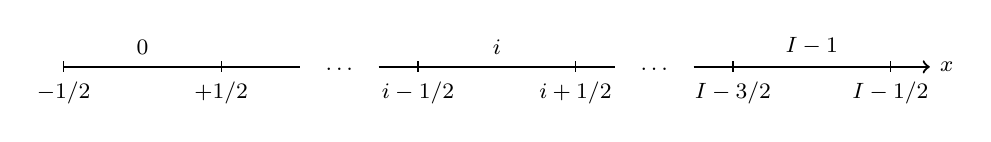
\begin{tikzpicture}
	\tikzstyle{every node}=[font=\footnotesize]
	\draw[thick] (0,0) -- (3,0);
	\node[anchor=south] at (3.5cm,-5pt) {$\ldots$};
	\draw[thick] (4,0) -- (7,0);
	\node[anchor=south] at (7.5cm,-5pt) {$\ldots$};
	\draw[thick,->] (8,0) -- (11,0) node[anchor=west] {$x$};

	\draw ( 0 cm,2pt) -- ( 0 cm,-2pt) node[anchor=north] {$-1/2$};
	\node[anchor=south] at (1cm,1pt) {0};
	\draw ( 2 cm,2pt) -- ( 2 cm,-2pt) node[anchor=north] {$+1/2$};

	\draw ( 4.5 cm,2pt) -- ( 4.5 cm,-2pt) node[anchor=north] {$i-1/2$};
	\node[anchor=south] at (5.5cm,1pt) {$i$};
	\draw ( 6.5 cm,2pt) -- ( 6.5 cm,-2pt) node[anchor=north] {$i+1/2$};

	\draw ( 8.5 cm,2pt) -- ( 8.5 cm,-2pt) node[anchor=north] {$I-3/2$};
	\node[anchor=south] at (9.5cm,1pt) {$I-1$};
	\draw ( 10.5 cm,2pt) -- ( 10.5 cm,-2pt) node[anchor=north] {$I-1/2$};
	\end{tikzpicture}
	\caption{Notation of the one-dimensional mesh.}
	\label{fig:mesh1D}
\end{figure}
%
Since the input diffusion coefficients are provided as node averaged, and they are always needed at interfaces, they are approximated by local volume averages:
\begin{equation}\label{eq:Ds}
D(x_{i+1/2},E) = \frac{\Delta x_i D(x_i,E) 
	+ \Delta x_{i+1} D(x_{i+1},E)}
{ \Delta x_i + \Delta x_{i+1}} \,\, .
\end{equation}

%
% ---------------------------------------------------
\subsection{The correction as a drift term}
\label{sec:corr-drift}

The new numerical corrections $\delta D$ are obtained on the interfaces using~\eq{eq:JD-dJ} to be used in the finite differences solver, together with the diffusive currents from~\eq{eq:JD-dJ}. Hence, the neutron balance resolved by the CMFD takes into account both types of currents $J_D$ and $\delta J$. %Non-linear iterations with new corrections given by $\delta J$ are needed because of their dependence on the unknown flux.
Hence, the one-dimensional multigroup neutron balance CMFD diffusion equations actually solved are
\begin{equation}\label{eq:diff1}
J_{D,g}^+(x) + \delta J_{D,g}^+(x) -  J_{D,g}^-(x) - \delta J_{D,g}^-(x) + \sigma_{g}\phi_g(x) =  \frac{\chi_g}{\keff}\sum\limits_{g'=1}^G\nu\sigma_{f,g'}(x)\phi_{g'}(x) + \sum\limits_{g'=1}^G\sigma_{s,g\leftarrow g'}\phi_{g'}(x) \,\, ,
\end{equation}
where $J_{D,g}^\pm (x)\equiv J_{D,g}(x_{i\pm 1/2})$.

Using the definitions in~\eqsand{eq:JD-dJ}{eq:Ds} and~\fig{fig:mesh1D}, the discretized form of~\eq{eq:diff1} is
\begin{eqnarray}\label{eq:FD_diff_full}
- 2D_{i+1/2}^g\frac{\phi_{i+1,g}-\phi_{i,g}}{\dx_{i+1} + \dx_i}
- 2\delta D_{i+1/2}^g\frac{\phi_{i+1,g}+\phi_{i,g}}{(\dx_{i+1}+\dx_i)}
&+& 2D_{i-1/2}^g\frac{\phi_{i,g}-\phi_{i-1,g}}{\dx_{i} + \dx_{i-1}}  
+ 2\delta D_{i-1/2}^g\frac{\phi_{i,g}+\phi_{i-1,g}}{(\dx_i+\dx_{i-1})} 
\nonumber \\
&+& \sigma_{i}^g \phi_{i,g} 
= \sum\limits_{g'=1}^G \sigma_{s,i}^{g\leftarrow g'}\phi_{i,g'}
+ \frac{\chi_g}{\keff}\sum\limits_{g'=1}^G
 \nu\sigma_{f,i}^{g'}\phi_{i,g'} 
\,\,.
\end{eqnarray}
Rearranging terms, one gets
\begin{eqnarray}\label{eq:FD_diff_org}
\left(
\frac{-D_{i-1/2}^g + \delta D_{i-1/2}^g }{\dx_{i-1}+\dx_{i}}
\right)
\phi_{i-1,g}
&+&\left[
\frac{D_{i+1/2}^g - \delta D_{i+1/2}^g}{\dx_{i+1}+\dx_i}
+\frac{D_{i-1/2}^g + \delta D_{i-1/2}^g}{\dx_{i}+\dx_{i-1}}
+\frac{\sigma_{i}^g}{2}
\right]
\phi_{i,g}
\nonumber \\
&+&\left(
\frac{-D_{i+1/2}^g -\delta D_{i+1/2}^g }{\dx_{i+1}+\dx_{i}}
\right)
\phi_{i+1,g} =
\frac{1}{2}q_{i,g}\,\, ,
\end{eqnarray}
where $q_{i,g}$ is the RHS of~\eq{eq:FD_diff_full}.

These equations can be formulated in operators notation according to
\begin{equation}\label{eq:op-not}
\mathcal{M}\Phi=\frac{1}{\keff}\mathcal{F}\Phi \,\, ,
\end{equation}
where $\mathcal{M}$ is the migration operator, whose entries are given by~\eq{eq:FD_diff_org} making it a three-diagonal banded matrix, and $\mathcal{F}$ is the neutron generation operator given by the second term in $q_{i,g}$ (see Eqs.~\ref{eq:FD_diff_full}-\ref{eq:FD_diff_org}). Note that $\mathcal{M}$ can be written as $\mathcal{M}=\mathcal{M}_0+\delta\mathcal{M}$ distinguishing the diffusion corrections from the constant diffusion coefficients derived from the transport problem. In the homogeneous case, $\mathcal{M}(x)=\mathcal{M}_0+\delta\mathcal{M}(x)$.
%
%Eq.~\eqref{eq:op-not} is solved using the power iteration algorithm, where the within-group equation is noted as $\mathcal{A}_g(x)\Phi_g(x)=\frac{1}{\keff}Q_g(x)$, where $\mathcal{A}_g(x)=\mathcal{A}_{g,0}+\delta\mathcal{A}_g(x)$.
%
% ---------------------------------------------------
\subsection{Evaluation of the currents by the integral form of the transport equation}
\label{sec:calc-int-curr}

The numerical evaluation of the neutron current $J_g(x)$ at cell interfaces requires spatial integration of~\eq{eq:tot-J}. The neutron current at any interface can be calculated by considering separately contributions from all cells who are to the left or to the right of the interface. The current at a cell interface is discretized as follows
\begin{eqnarray}\label{eq:tot-J-disc}
J_g(x_{i+1/2}) &=& \sum\limits_{l=0}^\infty  \frac{2l+1}{2}
\sum\limits_{m=0}^{[l/2]}  h_m
\bigg\{
E_{n_{l,m}+1}[\mcL_g(0,x_{i+1/2})] \psi_{l,g}(0) 
+(-1)^{l+1} E_{n_{l,m}+1}[\mcL_g(x_{i+1/2},a)]\psi_{l,g}(a)  \nonumber \\
&+&
\sum\limits_{j=0}^i q_{l,g,j}\int\limits_{x_{j-1/2}}^{x_{j+1/2}} dx'
E_{n_{l,m}}[\mcL_g(x',x_{i+1/2})]
%\nonumber \\
%&&
+(-1)^{l+1} 
\sum\limits_{j=i+1}^{I-1} q_{l,g,j}\int\limits_{x_{j-1/2}}^{x_{j+1/2}} dx'
E_{n_{l,m}}[\mcL_g(x_{i+1/2},x')]
\bigg\}	\,\, , 
\end{eqnarray}
where $n_{l,m}\equiv l+2-2m$. The source $q_{l,g,j}$ is the $l$\tsup{th} angular moment of the volume-average within-group source in the cell $j$. The optical lengths show the subscript $g$ because they are evaluated with the corresponding total cross section $\sigma_g$. Note that for void boundary conditions, the boundary terms vanish by definition. The spatial integrals in~\eq{eq:tot-J-disc} can be solved analytically knowing that $E'_{n+1}(u)=-E_n(u)$~\cite{Gradshteyn-2007}. Using the notation in Fig.~\ref{fig:Xi}, the optical length between the right surfaces of cell $j$ and cell $i$ is
\begin{equation}\label{eq:psi_w_left_right}
\Xi^g_{i,j} \equiv \begin{cases}
\Xi^g_{i\geqslant j} = \sum\limits_{k=j+1}^i \sigma_{g,k}\Delta x_k 
& x\geqslant x' \quad (i\geqslant j) \\
\Xi^g_{i<j} = \sum\limits_{k=i+1}^{j-1} \sigma_{g,k}\Delta x_k & x<x' \quad (i<j)\,\, .
\end{cases} 
\end{equation} 

\begin{figure}[htbp!] 
	\centering
	For $x\geqslant x'$.	
	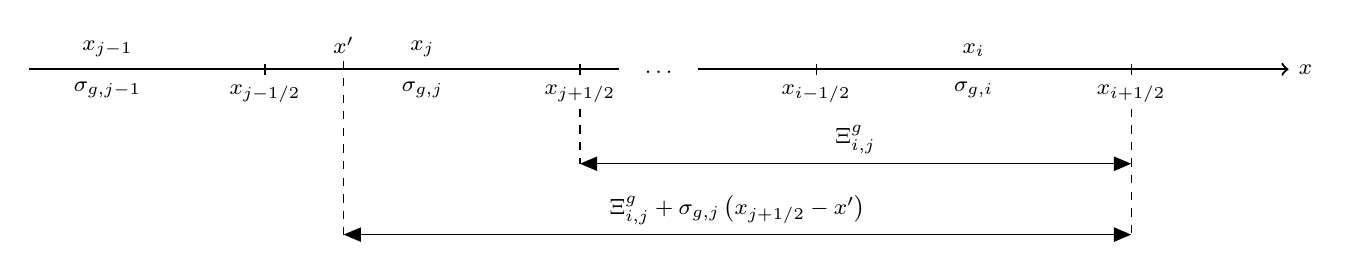
\begin{tikzpicture}
	\tikzstyle{every node}=[font=\footnotesize]
	\draw[thick] (0,0) -- (7.5,0);
	\draw[thick,->] (8.5,0) -- (16,0) node[anchor=west] {$x$};
	
	
	\node[anchor=south] at (1cm,1pt) {$x_{j-1}$};
	\node[anchor=north] at (1cm,-1pt) {$\sigma_{g,j-1}$};
	
	\draw ( 3 cm,2pt) -- ( 3 cm,-2pt) node[anchor=north] {$x_{j-1/2}$};
	\node[anchor=south] at (5cm,1pt) {$x_j$};
	\node[anchor=north] at (5cm,-1pt) {$\sigma_{g,j}$};
	\draw ( 7 cm,2pt) -- ( 7 cm,-2pt) node[anchor=north] {$x_{j+1/2}$};
	
	\node[anchor=south] at (8cm,-5pt) {$\ldots$};
	
	%\node[anchor=south] at (9cm,1pt) {$x_{j-1}$};
	
	\draw ( 10 cm,2pt) -- ( 10 cm,-2pt) node[anchor=north] {$x_{i-1/2}$};
	\node[anchor=south] at (12cm,1pt) {$x_{i}$};
	\node[anchor=north] at (12cm,-1pt) {$\sigma_{g,i}$};
	%\node[anchor=south] at (16.5cm,1pt) {$x_{j+1/2}$};
	\draw ( 14 cm,2pt) -- ( 14 cm,-2pt) node[anchor=north] {$x_{i+1/2}$};
	
	\node[anchor=south] at (4cm,2pt) {$x'$};
	
	% ------------------- Vertical dashed lines ------------------- %
	\draw [dashed] ( 7 cm, -0.5cm) -- ( 7 cm,-1.2cm);
	\draw [dashed] ( 14 cm, -0.5cm) -- ( 14 cm,-2.1cm);
	\draw [dashed] ( 4 cm, 0.1cm) -- ( 4 cm,-2.1cm);	
	
	% ------------------- Horizontal arrows + text ------------------- %
	\draw[>=triangle 45, <->] (7cm,-1.2cm) -- (14cm,-1.2cm);
	\node[anchor=south] at (10.5cm,-1.2cm) {$\Xi_{i,j}^g$};
	
	\draw[>=triangle 45, <->] (4cm,-2.1cm) -- (14cm,-2.1cm);
	\node[anchor=south] at (9cm,-2.1cm) {$\Xi_{i,j}^g + \sigma_{g,j}\left(x_{j+1/2} - x'\right)$};
	
	\end{tikzpicture}
	\bigbreak
	\bigbreak
	For $x<x'$.
	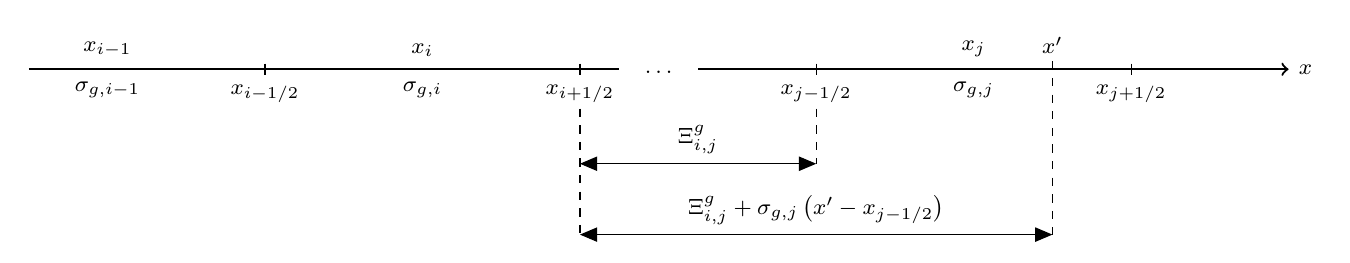
\begin{tikzpicture}
	\tikzstyle{every node}=[font=\footnotesize]
	\draw[thick] (0,0) -- (7.5,0);
	\draw[thick,->] (8.5,0) -- (16,0) node[anchor=west] {$x$};
	
	\node[anchor=south] at (1cm,1pt) {$x_{i-1}$};
	\node[anchor=north] at (1cm,-1pt) {$\sigma_{g,i-1}$};
	
	\draw ( 3 cm,2pt) -- ( 3 cm,-2pt) node[anchor=north] {$x_{i-1/2}$};
	\node[anchor=south] at (5cm,1pt) {$x_i$};
	\node[anchor=north] at (5cm,-1pt) {$\sigma_{g,i}$};
	\draw ( 7 cm,2pt) -- ( 7 cm,-2pt) node[anchor=north] {$x_{i+1/2}$};
	
	\node[anchor=south] at (8cm,-5pt) {$\ldots$};
	
	%\node[anchor=south] at (9cm,1pt) {$x_{j-1}$};
	
	\draw ( 10 cm,2pt) -- ( 10 cm,-2pt) node[anchor=north] {$x_{j-1/2}$};
	\node[anchor=south] at (12cm,1pt) {$x_{j}$};
	\node[anchor=north] at (12cm,-1pt) {$\sigma_{g,j}$};
	%\node[anchor=south] at (16.5cm,1pt) {$x_{j+1/2}$};
	\draw ( 14 cm,2pt) -- ( 14 cm,-2pt) node[anchor=north] {$x_{j+1/2}$};
	
	\node[anchor=south] at (13cm,2pt) {$x'$};
	
	% ------------------- Vertical dashed lines ------------------- %
	\draw [dashed] ( 7 cm, -0.5cm) -- ( 7 cm,-2.1cm);
	\draw [dashed] ( 10 cm, -0.5cm) -- ( 10 cm,-1.2cm);
	\draw [dashed] ( 13 cm, 0.1cm) -- ( 13 cm,-2.1cm);	
	
	% ------------------- Horizontal arrows + text ------------------- %
	\draw[>=triangle 45, <->] (7cm,-1.2cm) -- (10cm,-1.2cm);
	\node[anchor=south] at (8.5cm,-1.2cm) {$\Xi_{i,j}^g$};
	
	\draw[>=triangle 45, <->] (7cm,-2.1cm) -- (13cm,-2.1cm);
	\node[anchor=south] at (10cm,-2.1cm) {$\Xi_{i,j}^g + \sigma_{g,j}\left(x'-x_{j-1/2}\right)$};
	\end{tikzpicture}
	\bigbreak
	\caption{Notation for numerical evaluation of interface currents by the integral form of the transport equation.}
	\label{fig:Xi}
\end{figure}

Substituting 
\begin{equation}\label{eq:usub}
u = \begin{cases}
\Xi^g_{i\geqslant j} + \sigma_{g,j}(x_{j+1/2}-x') & x'\leqslant x \quad (j\leqslant i) \\
\Xi^g_{i<j} + \sigma_{g,j}(x'-x_{j-1/2}) & x'>x \quad (j>i)\,\, ,
\end{cases}
\end{equation} 
and integrating the $E_{n_{l,m}}$ terms in~\eq{eq:tot-J-disc} yields
\begin{eqnarray}\label{eq:E-int}
\int_{x_{j-1/2}}^{x_{j+1/2}}  dx'
E_{n_{l,m}}[\mcL_g(x',x_{i+1/2})] &=& \frac{1}{\sigma_{g,j}}
	\left[
	E_{n_{l,m}+1}(\Xi^g_{i\geqslant j}) 
	- E_{n_{l,m}+1}(\Xi^g_{i\geqslant j	}+\sigma_{g,j}\Delta x_j)
	\right] \nonumber \\
	&=&
	\frac{1}{\sigma_{g,j}}
	\left\{
	E_{n_{l,m}+1}\left[
	\mcL_g(x_{j+1/2},x_{i+1/2}) \right] 
	- E_{n_{l,m}+1}\left[
	\mcL_g(x_{j-1/2},x_{i+1/2})
	\right] 
	\right\} \nonumber \\	
\int_{x_{j-1/2}}^{x_{j+1/2}} dx'
E_{n_{l,m}}[\mcL_g(x_{i+1/2},x')] &=& \frac{1}{\sigma_{g,j}}
\left[
E_{n_{l,m}+1}(\Xi^g_{i<j}) 
- E_{n_{l,m}+1}(\Xi^g_{i<j	}+\sigma_{g,j}\Delta x_j)
\right]\nonumber \\	
	&=&
\frac{1}{\sigma_{g,j}}
\left\{
E_{n_{l,m}+1}\left[
\mcL_g(x_{i+1/2},x_{j-1/2}) \right] 
- E_{n_{l,m}+1}\left[
\mcL_g(x_{i+1/2},x_{j+1/2})
\right]
\right\}
\,\, .
\end{eqnarray}
Hence, the interface currents can be written as
\begin{eqnarray}\label{eq:tot-J-disc2}
J_g(x_{i+1/2}) &=& \sum\limits_{l=0}^\infty  \frac{2l+1}{2}
\sum\limits_{m=0}^{[l/2]}  h_m
\bigg\{
E_{n_{l,m}+1}[\mcL_g(0,x_{i+1/2})] \psi_{l,g}(0) 
+(-1)^{l+1} E_{n_{l,m}+1}[\mcL_g(x_{i+1/2},a)]\psi_{l,g}(a)  \nonumber \\
&+&
\sum\limits_{j=0}^i \frac{q_{l,g,j}}{\sigma_{g,j}} 
\left\{
E_{n_{l,m}+1}\left[
\mcL_g(x_{j+1/2},x_{i+1/2}) \right] 
- E_{n_{l,m}+1}\left[
\mcL_g(x_{j-1/2},x_{i+1/2})
\right] 
\right\}
\nonumber \\
&+&(-1)^{l+1} 
\sum\limits_{j=i+1}^{I-1} \frac{q_{l,g,j}}{\sigma_{g,j}} 
\left\{
E_{n_{l,m}+1}\left[
\mcL_g(x_{i+1/2},x_{j-1/2}) \right] 
- E_{n_{l,m}+1}\left[
\mcL_g(x_{i+1/2},x_{j+1/2})
\right]
\right\}
\bigg\}	\,\, . 
\end{eqnarray}
Note that for the isotropic case ($l=0$) Eq.~\eqref{eq:tot-J-disc2} reduces  to
\begin{eqnarray}\label{eq:tot-J-disc2-l=0}
J_g(x_{i+1/2}) &=& \frac{1}{2}
\bigg\{
E_3[\mcL_g(0,x_{i+1/2})] \psi_{0,g}(0) 
- E_3[\mcL_g(x_{i+1/2},a)]\psi_{0,g}(a)  \nonumber \\
&&+
\sum\limits_{j=0}^i \frac{q_{0,g,j}}{\sigma_{g,j}} 
\left\{
E_3\left[
\mcL_g(x_{j+1/2},x_{i+1/2}) \right] 
- E_3\left[
\mcL_g(x_{j-1/2},x_{i+1/2})
\right] 
\right\}
\nonumber \\
&&-
\sum\limits_{j=i+1}^{I-1} \frac{q_{0,g,j}}{\sigma_{g,j}} 
\left\{
E_3\left[
\mcL_g(x_{i+1/2},x_{j-1/2}) \right] 
- E_3\left[
\mcL_g(x_{i+1/2},x_{j+1/2})
\right]
\right\}
\bigg\}	\nonumber \\
&=&\frac{1}{2}
\bigg\{
E_3[\mcL_g(0,x_{i+1/2})] \psi_{0,g}(0) 
- E_3[\mcL_g(x_{i+1/2},a)]\psi_{0,g}(a)  \nonumber \\
&&+
\sum\limits_{j=0}^{I-1} \frac{q_{0,g,j}}{\sigma_{g,j}} 
\left\{
E_3\left[
\mcL_g(x_{j+1/2},x_{i+1/2}) \right] 
- E_3\left[
\mcL_g(x_{j-1/2},x_{i+1/2})
\right] 
\right\}\text{sign}(i-j)
\bigg\}
\,\, . 
\end{eqnarray}
These transfer probabilities $E_{n_{l,m}}[\tau_g(x_i,x_j)]$ are pre-calculated once and are stored in a multi-dimensional array.

%
% ---------------------------------------------------
\subsection{Boundary conditions}
\label{sec:BC}
A generalized form for the boundary condition (at the left) follows as
\begin{equation}\label{eq:BC}
J_D(x=0) = -D_0\frac{\phi_0}{\Delta x_0/2 + \zeta} \,\, ,
\end{equation} 
where $\zeta$ is the extrapolation length in case of vacuum. The Marshak boundary conditions are reproduced by $\zeta=2D$, but the more accurate value $\zeta\approx 2.13D$ is taken to match transport with better agreement~\cite{Lamarsh-1966}. Reflection can be reproduced by $\zeta\rightarrow\infty$, whereas the condition of zero-flux is realized by $\zeta=0$. 
%
The quantity $\delta J$ at the boundary takes the simpler form of $\delta J = -\delta D_{-1/2}\phi_0$, without dividing by the spatial width, since no particular extrapolation length is appropriate for the correction. The expression for the right boundary is straightforward, implying a non-negative current. One should recall that the diffusion coefficient remains constant throughout the calculation, and so is the extrapolated distance. Only $\delta D$ is recalculated and the correction is actually implemented through the currents, i.e., $J_{tr} = J_D + \delta J$.

%
% ---------------------------------------------------
\subsection{The Ronen iterative scheme}
\label{sec:RM-scheme}

The Ronen algorithm is described as follows (see Fig.~\ref{fig:RM-algo}):
\begin{enumerate}
	\item\label{it:init} Initialize - the algorithm receives the geometry and the cross sections of the problem as input. At this stage, the corrections to the diffusion coefficients $\delta D^{(0)}(x,E)$ are set to zero and the initial pure-diffusion operator $\mathcal{A}_0(E)$ is constructed. Initial guesses for the flux $\phi^{(0)}(x,E)$ and multiplication factor $k^{(0)}_\texttt{eff}$ are set.
	\item\label{it:DF-solve} Diffusion Solver - a one-dimensional multigroup diffusion solver is executed until convergence using the diffusion corrections from the previous iteration $\delta D^{(k)}(x,E)$ through the diffusion operator $\mathcal{A}^{(k)}(x,E)=\mathcal{A}_0(E)+\delta A^{(k)}(x,E)$. The results are an updated estimation of the diffusion flux $\phi^{(k)}(x,E)$ and the multiplication factor $k^{(k)}_\texttt{eff}$.
	\item\label{it:Js} Calculate Currents - using the updated diffusion flux $\phi^{(k)}(x,E)$, both the diffusion current $J^{(k)}_D(x,E)$ (Eq.~\ref{eq:JD-dJ}) and the transport current $J^{(k)}_\texttt{tr}(x,E)$ (Eq.~\ref{eq:tot-J}) are calculated.
	\item\label{it:dD} Calculate corrections - the diffusion correction $\delta D^{(k+1)}(x,E)$ (Eq.~\ref{eq:JD-dJ}) is obtained using $\delta J^{(k)}(x,E)$ and Eq.~\eqref{eq:JD-dJ}.
	\item\label{it:dA} Update diffusion coefficients - reconstruct the diffusion operator $\mathcal{A}^{(k+1)} = \mathcal{A}_0+\delta \mathcal{A}^{(k+1)}$ (Eq.~\ref{eq:FD_diff_org}).
	\item\label{it:conv} If flux and eigenvalue are not converged, go to step~\ref{it:DF-solve}.
\end{enumerate}

\begin{figure}[htbp!] 
	\centering
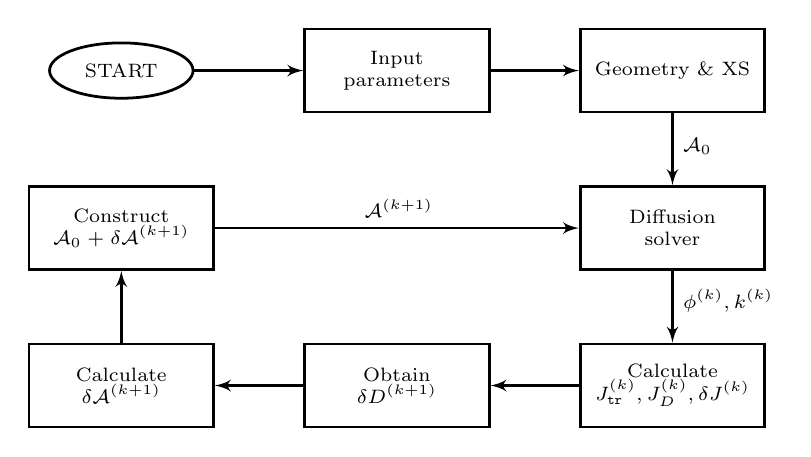
\begin{tikzpicture}[font=\scriptsize]
% Place nodes
	\node [cloud] 					 			(start) {START};
	\node [block, right of=start, xshift=0cm,yshift=0cm] (input) {Input\\parameters};
	\node [block, right of=input, xshift=0cm,yshift=0cm] (geoXS) {Geometry \& XS};
	\node [block, below of=geoXS, xshift=0cm,yshift=1.5cm] (Diff)  {Diffusion\\solver};
	\node [block, below of=Diff, xshift=0cm,yshift=1.5cm] (J)  {Calculate $J^{(k)}_{\texttt{tr}},J^{(k)}_D,\delta J^{(k)}$};
	\node [block, left  of=J,    xshift=0cm,yshift=0cm] (dD) {Obtain\\$\delta D^{(k+1)}$};
	\node [block, left  of=dD,   xshift=0cm,yshift=0cm](dA) {Calculate\\$\delta \mathcal{A}^{(k+1)}$};
	\node [block, above of=dA,   xshift=0cm,yshift=-1.5cm] (Anew) {Construct\\$\mathcal{A}_0+\delta \mathcal{A}^{(k+1)}$};

% Draw edges
	\path [line] (start) -- (input);
	\path [line] (input) -- (geoXS);
	\path [line] (geoXS) -- node[anchor= south west,yshift=-0.2cm]{$\mathcal{A}_0$}(Diff);
	\path [line] (Diff)  -- node[anchor= south west,yshift=-0.2cm]{$\phi^{(k)},k^{(k)}$}(J);
	\path [line] (J)  -- node[anchor= north]{}(dD);
	\path [line] (dD) -- node[anchor= north]{}(dA);
	\path [line] (dA)  -- node[anchor= north]{}(Anew);
	\path [line] (Anew)  -- node[near end,anchor= south west,xshift=-1.7cm]{$\mathcal{A}^{(k+1)}$}(Diff);

\end{tikzpicture}
	\caption{A flow chart of the Ronen algorithm.}
	\label{fig:RM-algo}
\end{figure}


%
% ---------------------------------------------------
\section{Results}
\label{sec:res}

Two one-dimensional test cases are considered, homogeneous and heterogeneous. The reference solutions are calculated using a Python3 discrete ordinates ($S_N$) code with $N=16$~\cite{Lewis-1984}. The diffusion solutions and the Ronen iterations are produced using original codes developed in Pyhton3. All thresholds are set to 1E-6 and no (over/under)-relaxation is done. The initial diffusion coefficient is set to $D=(3\sigma_{tr})^{-1}=(3\sigma)^{-1}$. Void boundary conditions are used at the edges of the slab, which are implemented for the diffusion solver in the form of a group-dependent extrapolated distance, i.e., $d_g = 2.13 D_g$.

%
% ---------------------------------------------------
\subsection{Homogeneous case}
\label{sec:homog}

A homogeneous slab of width $a=21.5$ cm is considered, with the two-group macroscopic cross sections shown in Table~\ref{tab:xs} (taken from~\cite{Tomatis-2011}). 
%
\begin{table}[!htbp]	
	\centering
	\caption{Two-group macroscopic cross sections [cm\tsup{-1}] used for the homogeneous case~\cite{Tomatis-2011}.}
	\label{tab:xs}
	\begin{tabular}{cccccc}
		%\midrule
		Group g &  $\sigma_{g}$ & \multicolumn{2}{c}{$\sigma_{s,0,g\leftarrow g'}$} & $\chi_g$ & $\nu\sigma_{f,g}$ \\ 
		\midrule
		1 & 5.3115$\times$10\tsup{-1} & 5.04664$\times$10\tsup{-1} & 2.03884$\times$10\tsup{-3} & 1 & 7.15848$\times$10\tsup{-3} \\
		%\midrule
		2 & 1.30058$\times$10\tsup{+0}& 1.62955$\times$10\tsup{-2} & 1.19134$\times$10\tsup{+0}	& 0 & 1.41284$\times$10\tsup{-1} \\
		%\midrule
	\end{tabular}
\end{table}

Table~\ref{tab:dx_drho} shows the reactivity differences as a function of mesh refinement using standard diffusion (with extrapolated length) and the Ronen method. The reactivity difference is given by $(\Delta\rho = 1/k_\texttt{ref} - 1/k_\texttt{D/RM})\times 10^5$, where $k_D$ and $k_{RM}$ are the multiplication factors of standard diffusion and the Ronen method, respectively. The reference $k_\texttt{ref}$ value from S\tsub{16} is 0.744417 ($I = 400$).  

\begin{table}[!htbp]
	\centering
	\caption{Reactivity differences as a function of mesh refinement using the Ronen method.}
	\label{tab:dx_drho}
	\begin{tabular}{lccccr}
		%\midrule
		$dx\quad (I)$ [cm]  &  $k_{\texttt{ref}}$ & $k_{\texttt{D}}$ & $\Delta\rho_\texttt{D}$ [pcm] & $k_{\texttt{RM}}$ & $\Delta\rho_\texttt{RM}$ [pcm]\\ 
		\midrule
		0.43 (50)     & 0.744307 & 0.741417 & -524 & 0.740552  & -681\\
		%\midrule
		0.215 (100)    & 0.744391 & 0.741355 & -550 & 0.743447 & -171\\
		%\midrule
		0.1075 (200)   & 0.744412 & 0.741339 & -557 & 0.744212 & -36\\
		%\midrule
		0.07167 (300) & 0.744416 & 0.741336 & -558 & 0.744356 & -11\\
		%\midrule
		0.05375 (400)  & 0.744417 & 0.741335 & -558 & 0.744407 & -2\\
		%\midrule
	\end{tabular}
\end{table}

A comparison of the fast and thermal fluxes, as calculated by the reference $S_N$ code, the RM code, and a standard multigroup diffusion without RM correction ($D_0$), is shown in Fig.~\ref{fig:slab-fluxes} for half-slab. The deviations (in [\%]) of the RM-corrected flux and the standard diffusion ($D_0$) flux from the reference $S_N$ flux is also shown in Fig.~\ref{fig:slab-fluxes-dev}. The corresponding Ronen method correction factors $\delta D$ are shown in Fig.~\ref{fig:slab-RM-corr-factor}. 

The deviation from the reference solution is decreased by the Ronen iterations from approximately 20\% near the boundary and 1\% at the slab center to 2\% and 0\%, respectively. 

%The diffusion and transport currents calculated using the converged Ronen solution are plotted in Fig.~\ref{fig:current}. The full slab solution exhibits anti-symmetry, as expected, whereas the corrected diffusion current exhibit non-trivial behavior near the boundary. 
%Fig.~\ref{fig:Dcoef} show the original standard diffusion coefficients ($D=(3\sigma_{tr})^{-1}$), The RM correction terms ($\delta D$), and the corrected (spatially-dependent) diffusion $D$. 

\begin{figure}[!htbp]
	\centering
	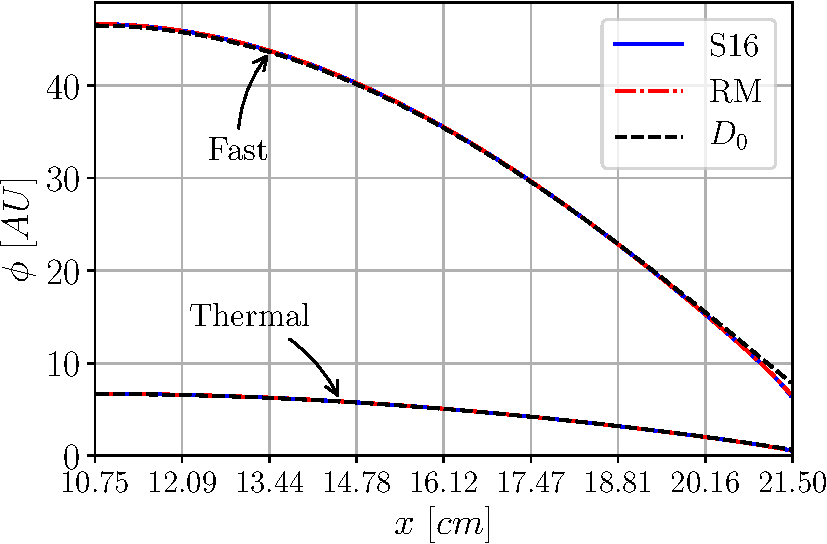
\includegraphics[width=0.65\linewidth]{Sn_Diff_RM_Tomatis2011.pdf}
	\caption{Comparison of the fluxes as calculated by the reference $S_N$ code, the RM code, and a standard multigroup diffusion without RM correction ($D_0$). Results shown here after 250 Ronen iterations.}
	\label{fig:slab-fluxes}		
\end{figure}

\begin{figure}[!htbp]
	\centering
	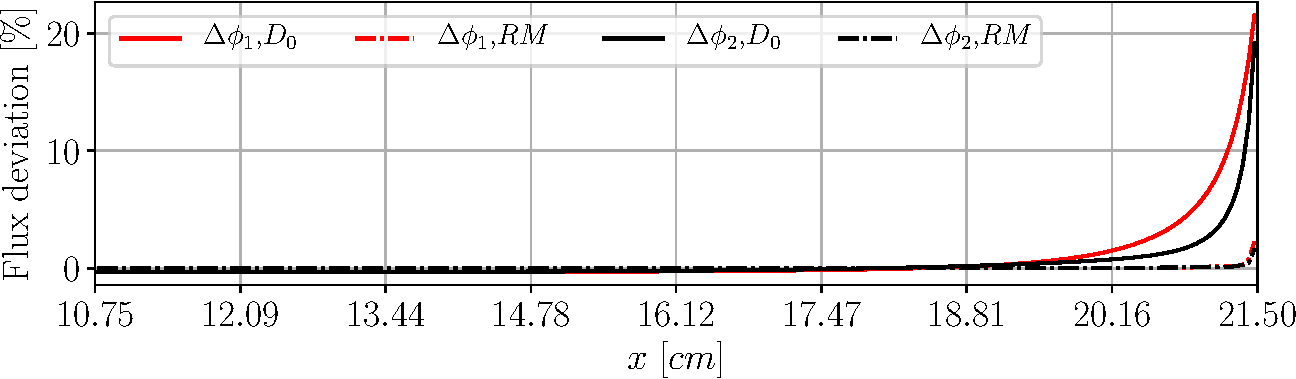
\includegraphics[width=0.65\linewidth]{flx_err_Tomatis2011_400_250.pdf}
	\caption{Deviation of the fluxes with respect to the reference solution after 250 Ronen iterations.}
	\label{fig:slab-fluxes-dev}
\end{figure}

\begin{figure}[!htbp]
	\centering
	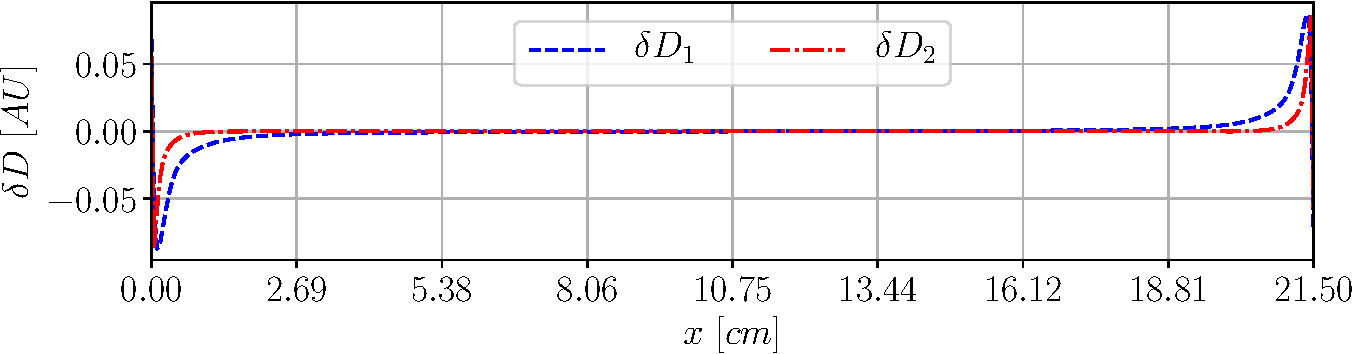
\includegraphics[width=0.65\linewidth]{dD_Tomatis2011_400_250it.pdf}
	\caption{The Ronen method correction factors ($\delta D$). Results shown here after 250 Ronen iterations.}
	\label{fig:slab-RM-corr-factor}
\end{figure}


%\begin{wrapfigure}{r}[0pt]{0.3\textwidth}
%	\centering
%	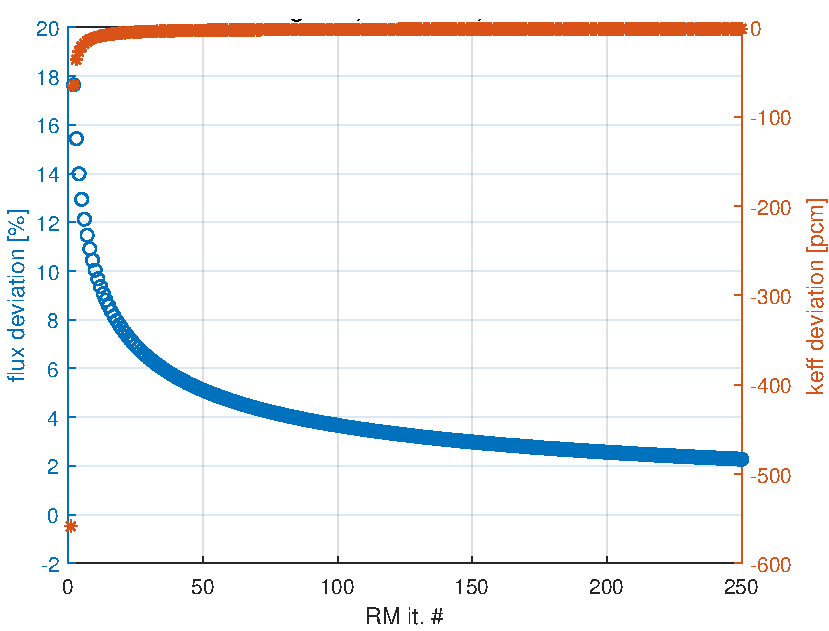
\includegraphics[width=\linewidth]{convergence.pdf}
%	\caption{Convergence of the flux (max deviation) and the criticality eigenvalue.}
%	\label{fig:conv}
%\end{wrapfigure} 

\begin{figure}[h!]
	% convergence
	\centering
	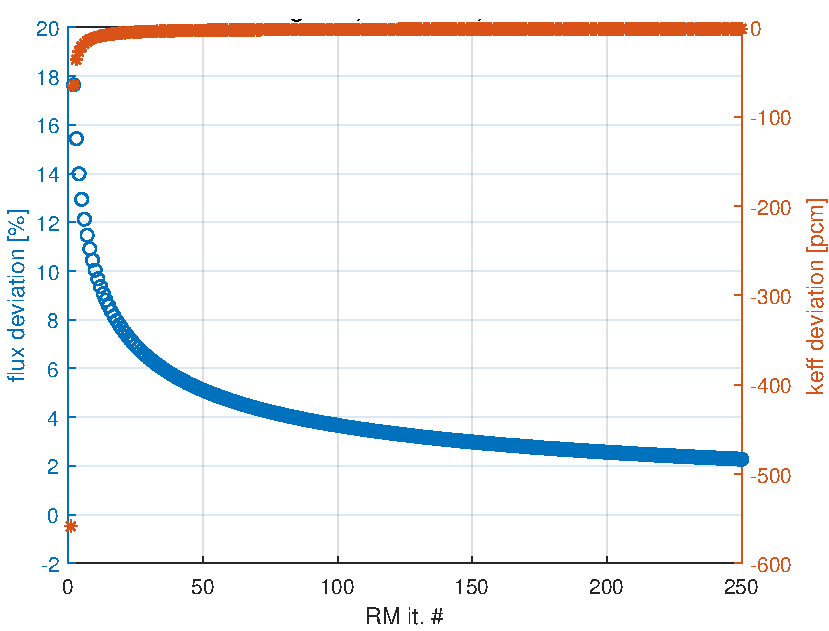
\includegraphics[width=0.4\linewidth]{convergence.pdf}
	\caption{Convergence of the flux (max deviation) and the criticality
		eigenvalue.}
	\label{fig:conv}
\end{figure}

The RM correction terms ($\delta D$) along the plane are shown in Fig.~\ref{fig:slab-RM-corr-factor}. It is clear that the diffusion correction assumes zero values at the slab center and exhibit non-trivial behavior near the boundary. The convergence of the flux (max deviation) and the criticality eigenvalue are shown in Fig.~\ref{fig:conv}. While the eigenvalue converges within a few iterations, the flux exhibit slow convergence near the boundaries. The spatial flux convergence between two successive Ronen iterations is shown in Fig.~\ref{fig:conv2} for the left half slab, according to $\Delta\phi = (\phi^{k-1}-\phi^k)/\phi^{k-1}$ [\%]. The spatial flux convergence of the Ronen iterations with respect to the reference $S_N$ solution for the left half slab is shown in Fig.~\ref{fig:conv3}.

% convergence
\begin{figure}[h!]
	\centering
	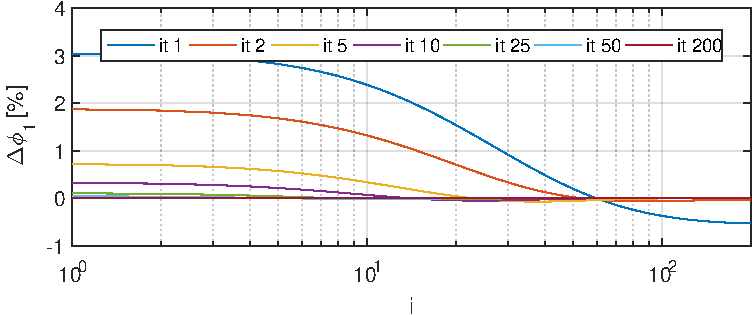
\includegraphics[width=0.48\linewidth]{flux_deviation_half_it_1.pdf}
	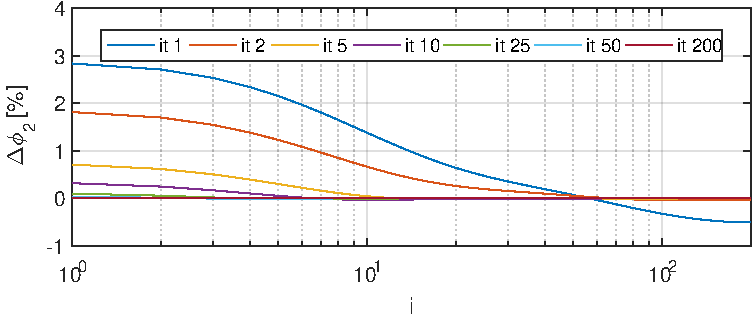
\includegraphics[width=0.48\linewidth]{flux_deviation_half_it_2.pdf}
	\caption{The spatial flux convergence between two successive Ronen iterations for the left half slab, according to $\Delta\phi = (\phi^{(k-1)}-\phi^{(k)})/\phi^{(k-1)}$ [\%].}
	\label{fig:conv2}
\end{figure}

% convergence
\begin{figure}[htbp!]
	\centering
	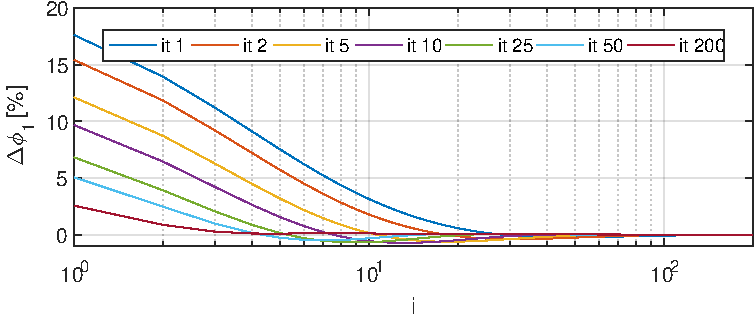
\includegraphics[width=0.48\linewidth]{flux_deviation_half_it_1_sn.pdf}
	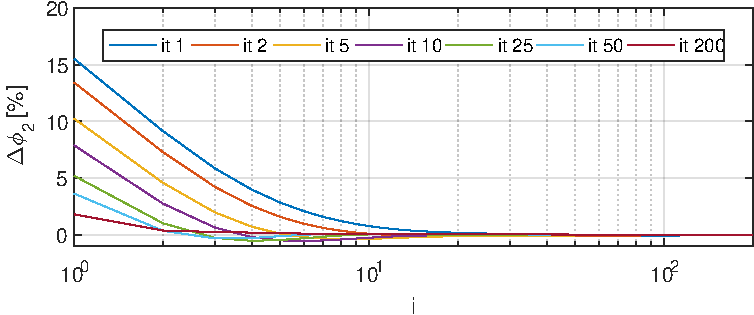
\includegraphics[width=0.48\linewidth]{flux_deviation_half_it_2_sn.pdf}
	\caption{The spatial flux convergence of the Ronen iterations with respect to the reference $S_N$ solution for the left half slab.}
	\label{fig:conv3}
\end{figure}

Notice the change of sign in the flux convergence $\Delta \phi$ in Fig.~\ref{fig:conv2} between the center (negative) and the boundary (positive) of the slab. The initial diffusion solution is smoother than the transport one. Hence, as can be seen in Fig.~\ref{fig:slab-fluxes}, the diffusion solution underestimates the peak flux at the center of the slab and overestimates the flux near the boundary. The Ronen iterations "push" the diffusion solution towards the transport one by increasing the flux level at the center of the slab and decreasing the flux level at the boundary. Hence, $\phi^{(k-1)}$ is smaller in the center and larger at the boundary comparing to $\phi^{(k)}$. This effect of the Ronen iterations produces less smooth flux shape with steeper gradients comparing to the diffusion solution.
%
% ---------------------------------------------------
\subsection{Heterogeneous case}
\label{subsec:heterog}

The heterogeneous benchmark defines three heterogeneous cores, each is 7 fuel assemblies long and comprised of four different fuel assemblies made of four different materials~\cite{Rahnema-1997}, as shown in Fig.~\ref{fig:hetro-core}. Material properties for each region of the assemblies are given in Table~\ref{tab:xs2}. Configuration 1 represents the least heterogeneous core with rather smooth flux gradients. On the contrary, configuration 3 represents the most heterogeneous core with the steepest flux gradients and can serve as a limiting case. Void boundary conditions are imposed on both ends of the core. 

\begin{figure}[htbp!] 
	\centering
	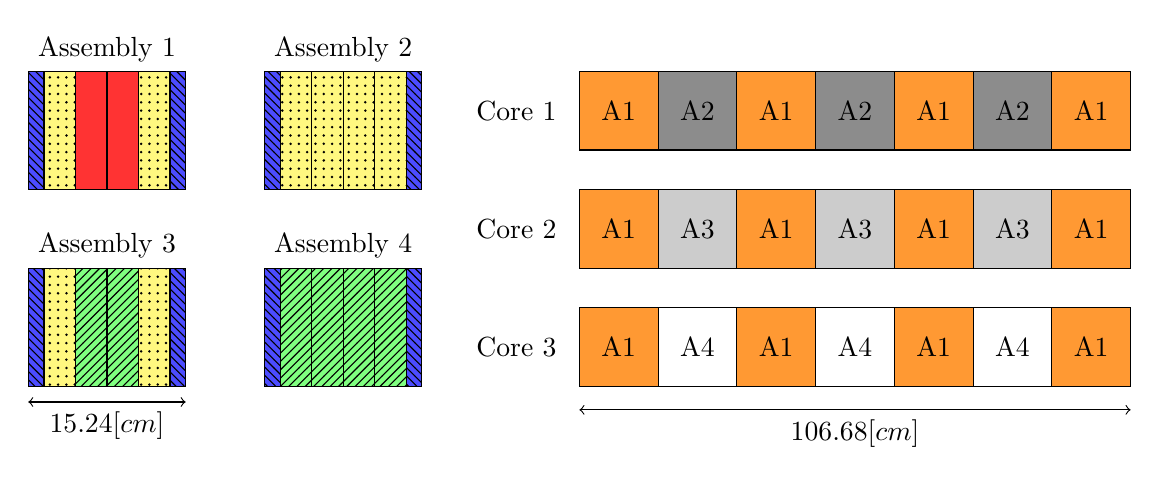
\begin{tikzpicture}
	% -------------- Assembly 1 --------------
	\node[above] at (-2,1.5) {Assembly 1};
	\draw[pattern=north west lines, preaction={fill=blue!70}] (-3,0)   rectangle (-2.8,1.5);
	\draw[pattern=dots, preaction={fill=yellow!50}] 		  (-2.8,0) rectangle (-2.4,1.5);
	\draw[fill=red!80] 										  (-2.4,0) rectangle (-2,1.5);
	\draw[fill=red!80]	  									  (-2,0)   rectangle (-1.6,1.5);
	\draw[pattern=dots, preaction={fill=yellow!50}] 		  (-1.6,0) rectangle (-1.2,1.5);
	\draw[pattern=north west lines, preaction={fill=blue!70}] (-1.2,0) rectangle (-1,1.5);
	% -------------- Assembly 2 --------------
	\node[above] at (1,1.5) {Assembly 2};
	\draw[pattern=north west lines, preaction={fill=blue!70}] (0,0)	  rectangle (0.2,1.5);
	\draw[pattern=dots, preaction={fill=yellow!50}] 		  (0.2,0) rectangle (0.6,1.5);
	\draw[pattern=dots, preaction={fill=yellow!50}] 		  (0.6,0) rectangle (1,1.5);
	\draw[pattern=dots, preaction={fill=yellow!50}] 		  (1,0)   rectangle (1.4,1.5);
	\draw[pattern=dots, preaction={fill=yellow!50}] 		  (1.4,0) rectangle (1.8,1.5);
	\draw[pattern=north west lines, preaction={fill=blue!70}] (1.8,0) rectangle (2,1.5);
	% -------------- Assembly 3 --------------
	\node[above] at (-2,-1) {Assembly 3};
	\draw[pattern=north west lines, preaction={fill=blue!70}]  (-3,-2.5)   rectangle (-2.8,-1);
	\draw[pattern=dots, preaction={fill=yellow!50}] 		   (-2.8,-2.5) rectangle (-2.4,-1);
	\draw[pattern=north east lines, preaction={fill=green!50}] (-2.4,-2.5) rectangle (-2,-1);
	\draw[pattern=north east lines, preaction={fill=green!50}] (-2,-2.5)   rectangle (-1.6,-1);
	\draw[pattern=dots, preaction={fill=yellow!50}] 		   (-1.6,-2.5) rectangle (-1.2,-1);
	\draw[pattern=north west lines, preaction={fill=blue!70}] (-1.2,-2.5)  rectangle (-1,-1);
	\draw [<->] (-3,-2.7) -- node[below]{$15.24[cm]$}	(-1,-2.7);
	% -------------- Assembly 4 --------------
	\node[above] at (1,-1) {Assembly 4};
	\draw[pattern=north west lines, preaction={fill=blue!70}]  (0,-2.5)    rectangle (0.2,-1); 
	\draw[pattern=north east lines, preaction={fill=green!50}] (0.2,-2.5)  rectangle (0.6,-1);
	\draw[pattern=north east lines, preaction={fill=green!50}] (0.6,-2.5)  rectangle (1,-1);
	\draw[pattern=north east lines, preaction={fill=green!50}] (1,-2.5)    rectangle (1.4,-1);
	\draw[pattern=north east lines, preaction={fill=green!50}] (1.4,-2.5)  rectangle (1.8,-1);
	\draw[pattern=north west lines, preaction={fill=blue!70}]  (1.8,-2.5)  rectangle (2,-1);
	% -------------- Core 1 --------------
	\node[] at (3.2,1) {Core 1};
	\draw [fill=orange!80]   (4,0.5)   rectangle node{A1} 	(5,1.5);
	\draw [fill=gray!90] 	 (5,0.5)   rectangle node{A2}	(6,1.5);
	\draw [fill=orange!80]   (6,0.5)   rectangle node{A1}	(7,1.5);
	\draw [fill=gray!90] 	 (7,0.5)   rectangle node{A2}	(8,1.5);
	\draw [fill=orange!80]   (8,0.5)   rectangle node{A1}	(9,1.5);
	\draw [fill=gray!90] 	 (9,0.5)   rectangle node{A2}	(10,1.5);
	\draw [fill=orange!80]   (10,0.5)  rectangle node{A1}	(11,1.5);
	% -------------- Core 2 --------------
	\node[] at (3.2,-0.5) {Core 2};
	\draw [fill=orange!80]   (4,-1)   rectangle node{A1}	(5,-0);
	\draw [fill=gray!40] 	 (5,-1)   rectangle node{A3}	(6,-0);
	\draw [fill=orange!80]   (6,-1)   rectangle node{A1}	(7,-0);
	\draw [fill=gray!40] 	 (7,-1)   rectangle node{A3}	(8,-0);
	\draw [fill=orange!80]   (8,-1)   rectangle node{A1}	(9,-0);
	\draw [fill=gray!40] 	 (9,-1)   rectangle node{A3}	(10,-0);
	\draw [fill=orange!80]   (10,-1)  rectangle node{A1}	(11,-0);
	% -------------- Core 3 --------------
	\node[] at (3.2,-2) {Core 3};
	\draw [fill=orange!80]  (4,-2.5)  rectangle node{A1} 	(5,-1.5);
	\draw [fill=white] 		(5,-2.5)  rectangle node{A4}	(6,-1.5);
	\draw [fill=orange!80]  (6,-2.5)  rectangle node{A1}	(7,-1.5);
	\draw [fill=white] 		(7,-2.5)  rectangle node{A4}	(8,-1.5);
	\draw [fill=orange!80]  (8,-2.5)  rectangle node{A1}	(9,-1.5);
	\draw [fill=white] 		(9,-2.5)  rectangle node{A4}	(10,-1.5);
	\draw [fill=orange!80]  (10,-2.5) rectangle node{A1}	(11,-1.5);
	\draw [<->] (4,-2.8) -- node[below]{$106.68[cm]$}	(11,-2.8);
	\end{tikzpicture}
	\caption{Schematic illustration of the fuel assemblies and core composition and geometry~\cite{Rahnema-1997}.}
	\label{fig:hetro-core}	
\end{figure}


\begin{table}[htbp!]	
	\centering
	\caption{Two-group macroscopic cross sections [cm\tsup{-1}] used for the heterogeneous case~\cite{Rahnema-1997}. Colors are in accordance with Fig.~\ref{fig:hetro-core}.} 
	\label{tab:xs2}
	\begin{tabular}{lcccccccr}
		Material&$\sigma_1$&$\sigma_2$&$\nu\sigma_{f,1}$&$\nu\sigma_{f,2}$&$\sigma_{s,1\leftarrow 1}$&$\sigma_{s,2\leftarrow 1}$&$\sigma_{s,2\leftarrow 2}$&$x[cm]$\\
		\midrule
		Water  (Blue)	&0.1890	 &1.4633  &0.0000	 &0.0000	 &0.1507   &0.0380		&1.4536		 &1.158\\
		Fuel 1 (Red)	&0.2263  &1.0119  &0.0067	 &0.1241	 &0.2006   &0.0161		&0.9355		 &3.231\\
		Fuel 2 (Yellow)	&0.2252  &0.9915  &0.0078	 &0.1542 	 &0.1995   &0.0156		&0.9014		 &3.231\\
		Fuel 3 (Green)	&0.2173  &1.0606  &0.0056	 &0.0187	 &0.1902   &0.0136		&0.5733 	 &3.231\\
	\end{tabular}
\end{table}

Table~\ref{tab:dx_drho2} shows the reactivity differences between standard diffusion (with extrapolated length) and the Ronen method (at increasing number of iterations) with respect to the reference solution for each of the three core configurations. The standard diffusion solution perform rather well for core 1 with deviation of 182 pcm, but fails for cores 2 and 3 with deviation of 773 and 3335 pcm, respectively. This is explained by the fact that cores 2 and 3 are more heterogeneous with respect to core 1. The Ronen method performs better than standard diffusion for all three cores, even after merely 10 iterations. Additional Ronen iterations further improve the estimated multiplication factor but less with milder changes.      

\begin{table}[!htbp]
	\centering
	\caption{Reactivity differences as a function of number of iterations using the Ronen method. 728 nodes.}
	\label{tab:dx_drho2}
	\begin{tabular}{lcccccr}
		%\midrule
		Method & \multicolumn{2}{c}{Core 1} & \multicolumn{2}{c}{Core 2} & \multicolumn{2}{c}{Core 3}  \\ 
		\midrule
		{}				& $\keff$& $\Delta\rho$ [pcm]& $\keff$	&$\Delta\rho$ [pcm]& $\keff$ &$\Delta\rho$ [pcm] \\
		$S_{16}$		&1.25614	&-			 &1.00094   &-				  &0.79878		&-		\\
		Diffusion		&1.25902	&182		 &0.99325	&-773			  &0.77805		&-3335	\\
		RM-10			&1.25677	&40			 &1.00107	&13			 	  &0.79824		&-85	\\
		RM-20			&1.25648	&22			 &1.00091	&-3			  	  &0.79837		&-64	\\
		RM-50			&1.25625	&7			 &1.00076	&-18			  &0.79839		&-61	\\
		RM-100			&1.25618	&3			 &1.00070	&-24			  &0.79838		&-62	\\		
	\end{tabular}
\end{table}

The two-group flux distribution across each core is shown in Fig.~\ref{fig:hetero-flux} for standard diffusion ($D_0$), Ronen method (RM) and the S16 reference solution. RM results are shown for 100 iterations and the spatial mesh spans 8 nodes in the water and 22 nodes in each fuel element. On a first glance, it is easy to see that standard diffusion fails to produce the steep flux gradients across material interfaces, especially between fuel and water. This is more pronounced for the fast flux, where even in core 1 it is not described correctly. 

\begin{figure}[htbp!]
	\centering
	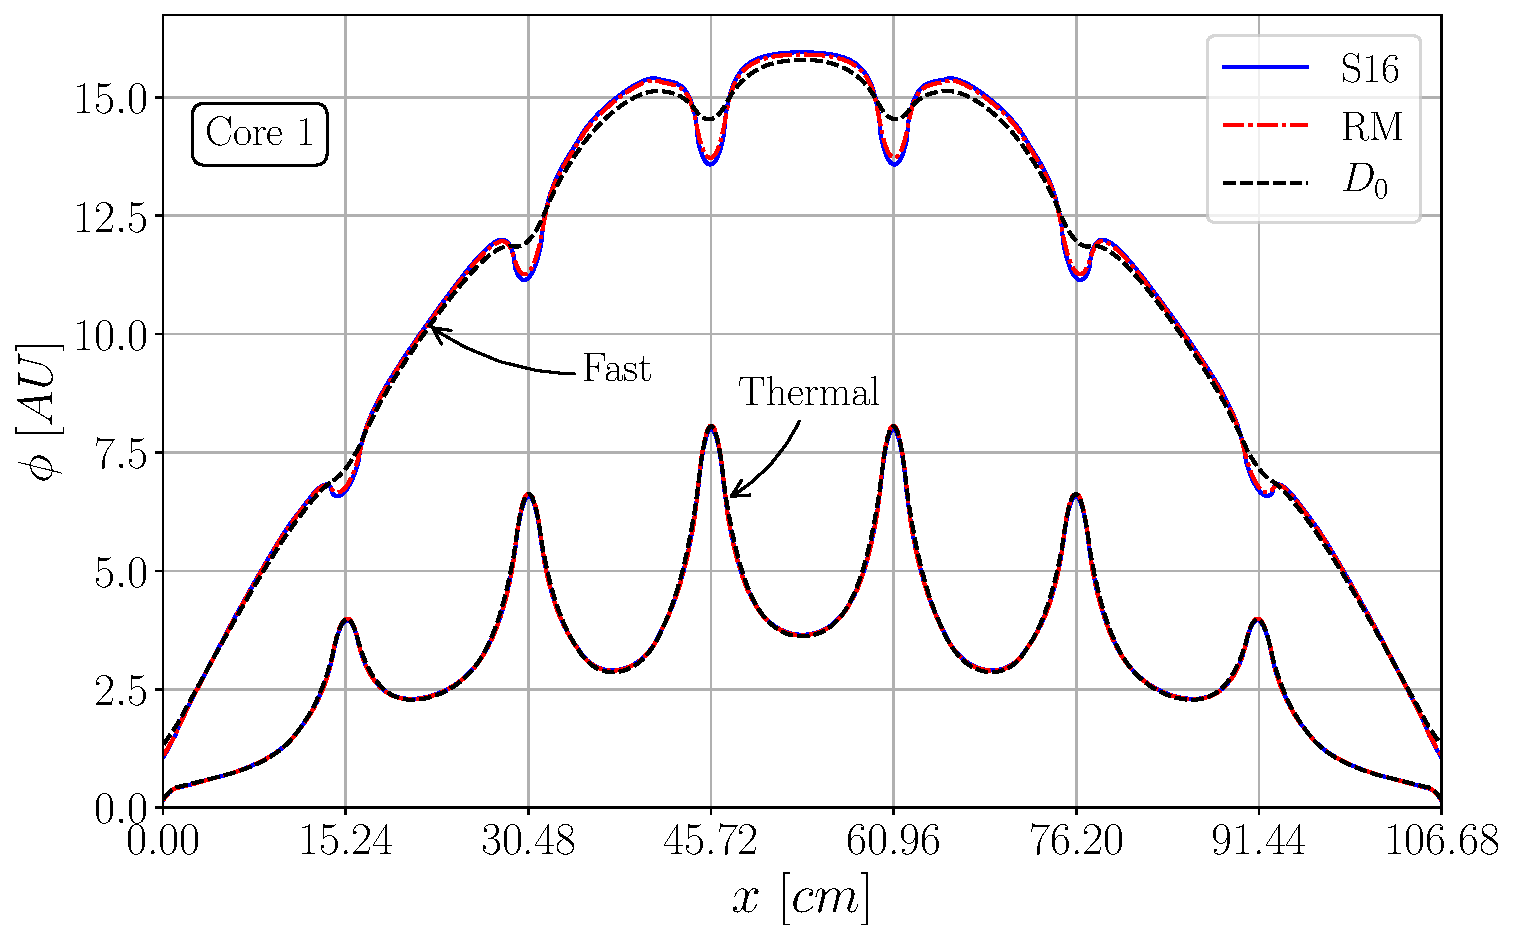
\includegraphics[width=0.49\linewidth]{Sn_Diff_RM_core_1.pdf}
	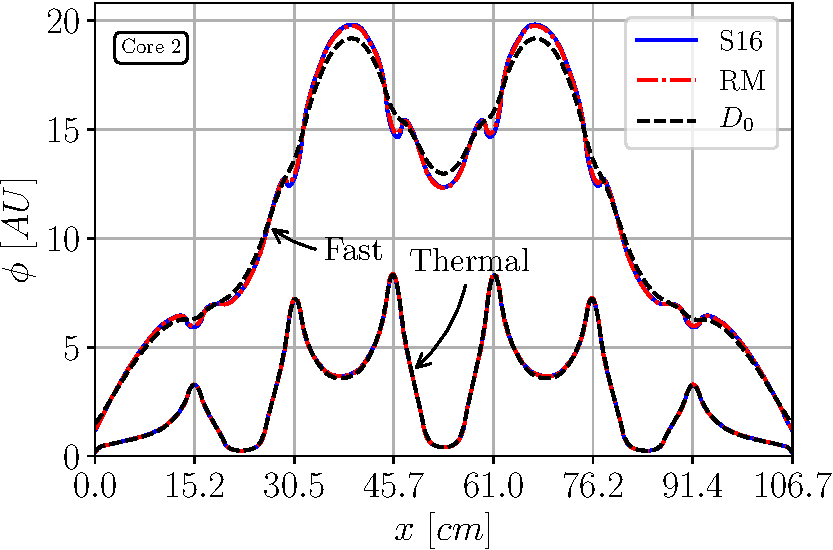
\includegraphics[width=0.49\linewidth]{Sn_Diff_RM_core_2.pdf}
	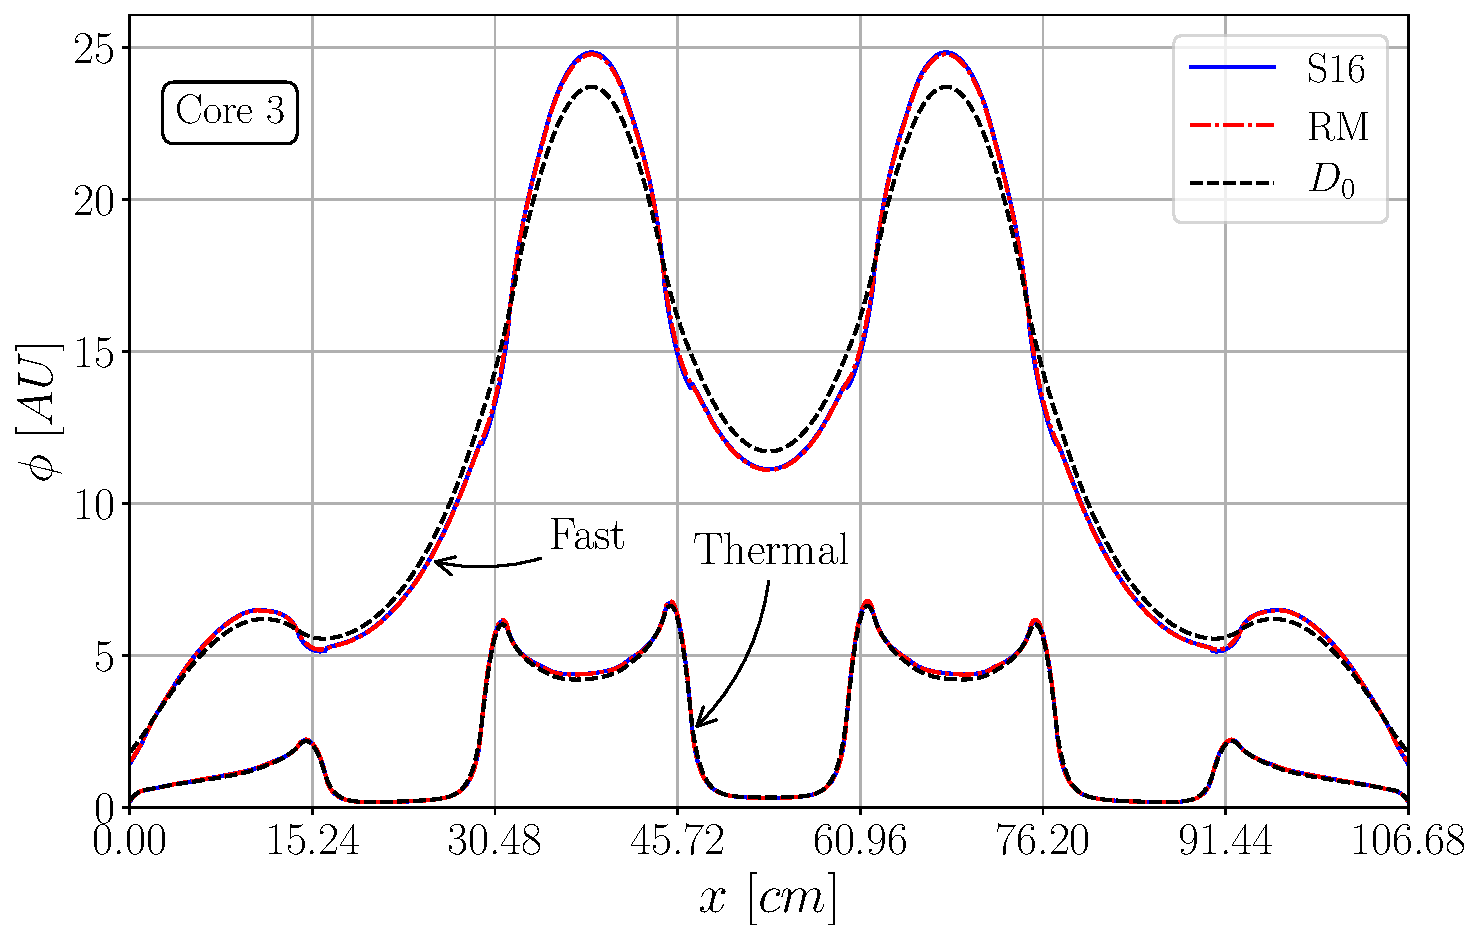
\includegraphics[width=0.49\linewidth]{Sn_Diff_RM_core_3.pdf}
	\caption{Fast and thermal flux for each core using standard diffusion ($D_0$), Ronen method (RM) and S16 reference solution. Vertical grid lines are located at assemblies interfaces. RM results are for 100 iterations and the spatial mesh spans 8 nodes in the water and 22 nodes in each fuel element.}
	\label{fig:hetero-flux}
\end{figure}

The fast and thermal flux deviation of standard diffusion ($D_0$) and Ronen method (RM) with respect to S16 reference solutions are shown for each core, in Fig.~\ref{fig:hetero-flux-dev}. The fast flux is poorly reproduced by standard diffusion, with up to $\sim$10\% deviations at the inner interfaces and $\sim$20\% at the outer boundaries (in agreement with the homogeneous case). Deviations of the thermal flux calculated by diffusion increase from $\sim$4\% to $\sim$10\% as the heterogeneity of the core increases. The deviations of the fast and thermal flux calculated by Ronen method are much smaller (practically negligible), and are smaller than $\sim$2\%. 

\begin{figure}[htbp!]
	\centering
	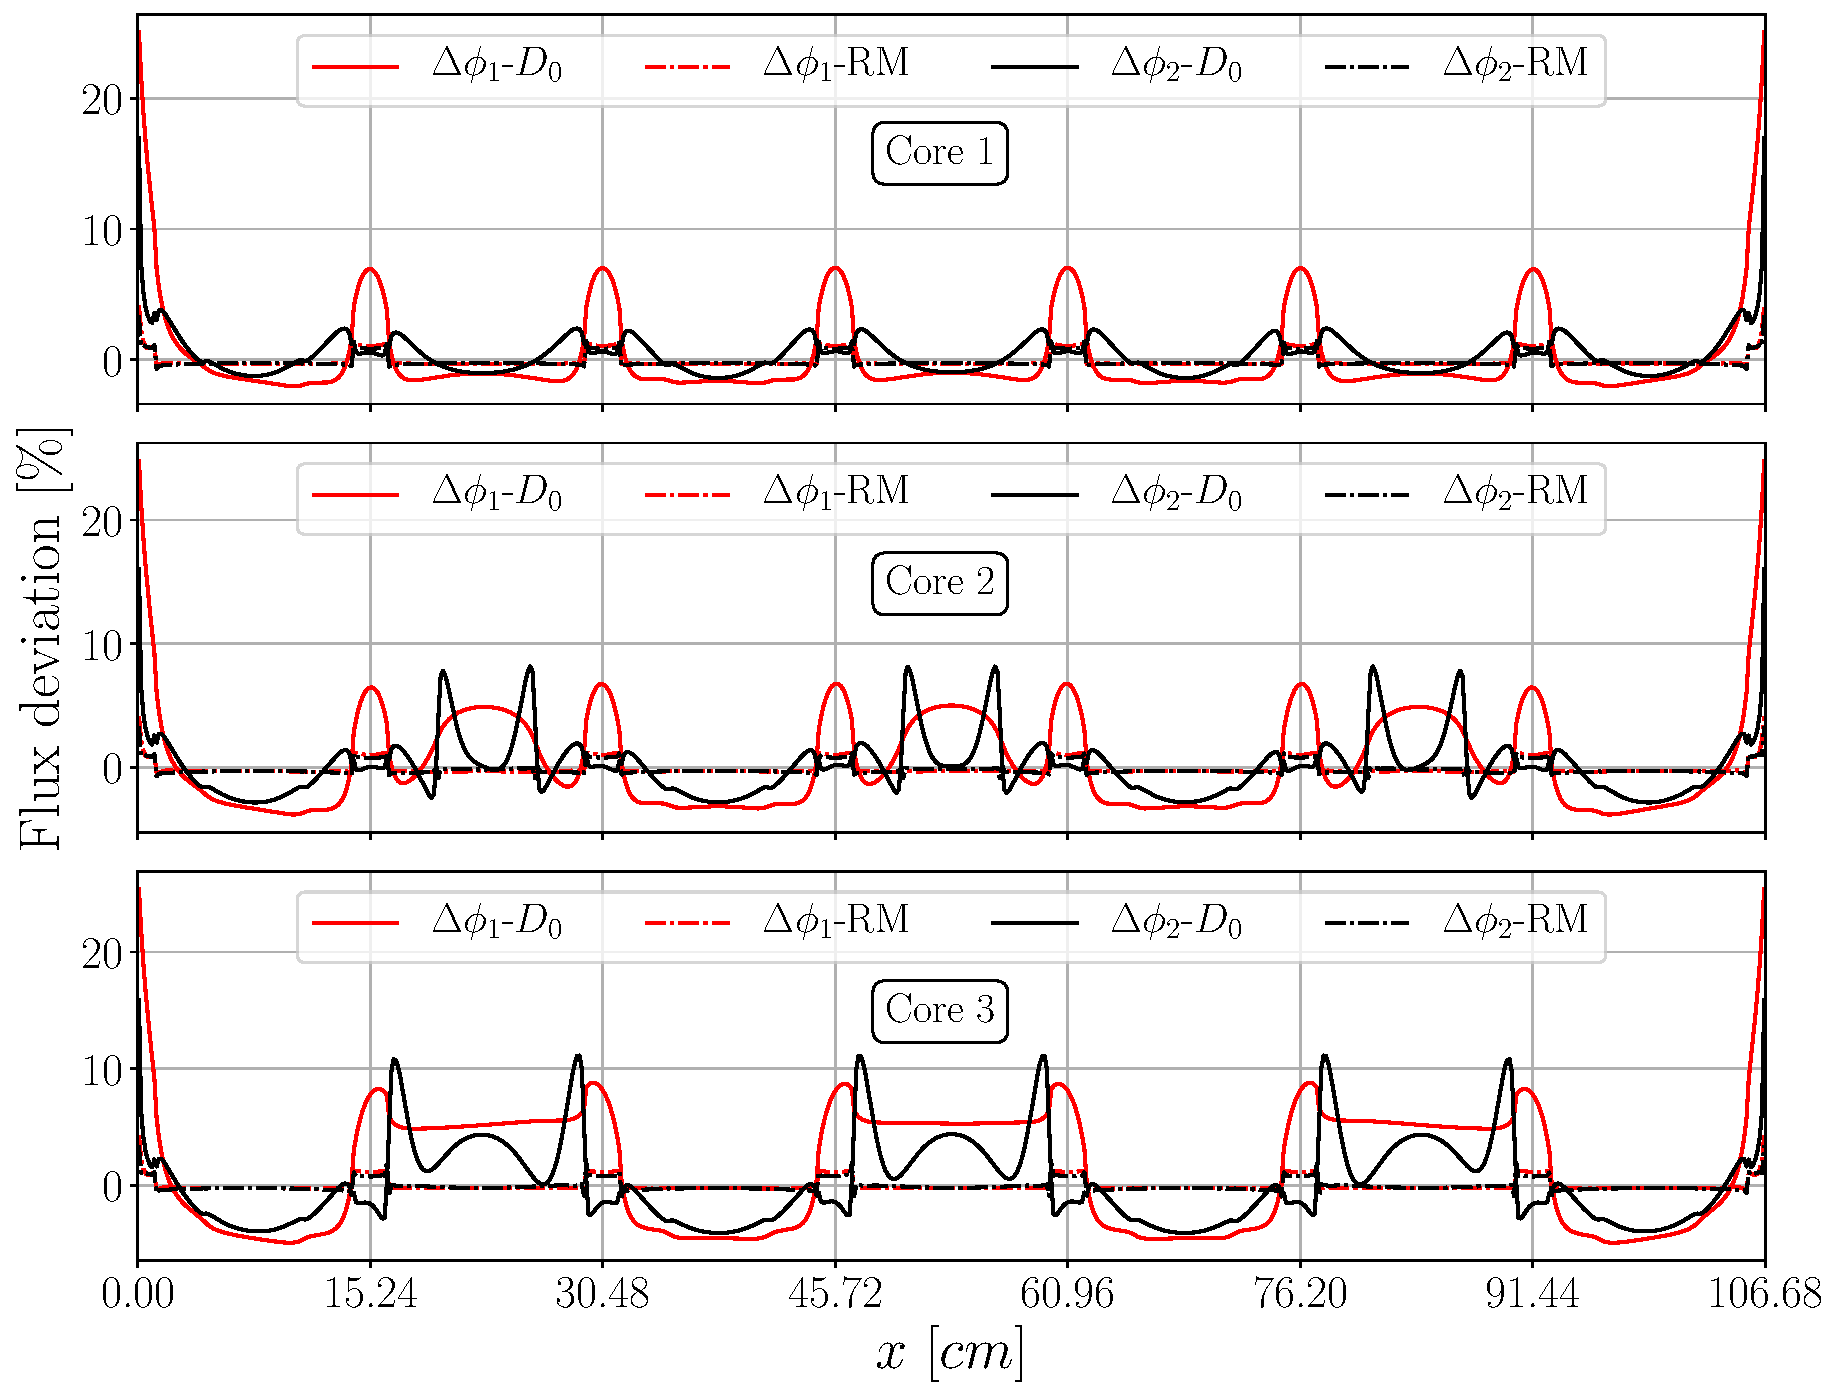
\includegraphics[width=0.75\linewidth]{flx_err_diff_C123.pdf}
	\caption{Fast and thermal flux deviation of standard diffusion ($D_0$) and Ronen method (RM) with respect to S16 reference solutions for each core. Vertical grid lines are located at assemblies interfaces. RM results are for 100 iterations and the spatial mesh spans 8 nodes in the water and 22 nodes in each fuel element.}
	\label{fig:hetero-flux-dev}
\end{figure}

It is illustrative to examine the spatial distribution of the Ronen method correction factors for the heterogeneous case. The behavior of the correction factor (Fig.~\ref{fig:Dcoef}) may seem a bit erratic, but can be explained. In regions where the flux gradients are small, the correction factors tend to vanish and actually produce solutions similar to standard diffusion. However, in regions where the flux gradients are steep, the correction factors do not vanish and play an important role in reproducing the correct flux shape.

\begin{figure}[htbp!]
	\centering
	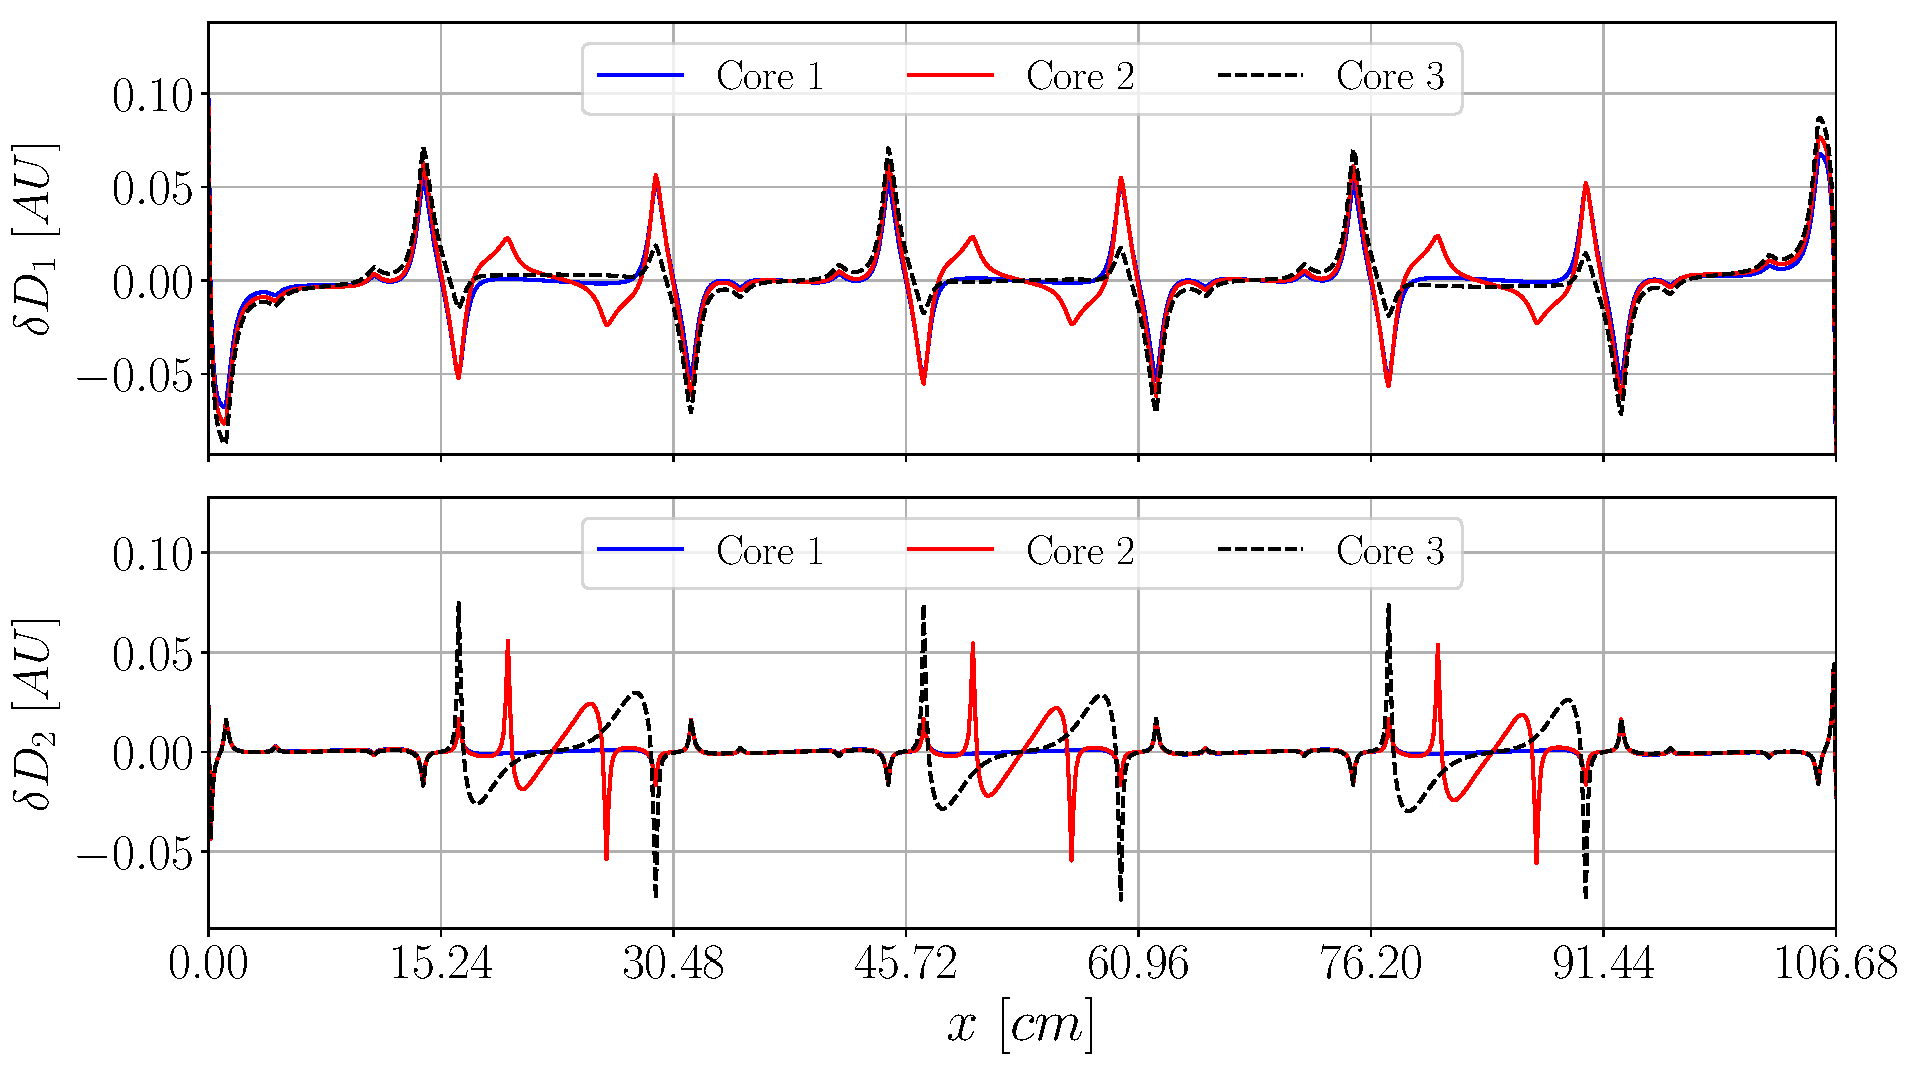
\includegraphics[width=0.75\linewidth]{RM_dD_100it_8_22_728_C123.pdf}
	\caption{Behavior of the Ronen method correction factor $dD$ along the core, for the fast and thermal fluxes. Vertical grid lines are located at assemblies interfaces, results are for 100 iterations and the spatial mesh spans 8 nodes in the water and 22 nodes in each fuel element.}
	\label{fig:Dcoef}
\end{figure}






%
% ---------------------------------------------------
\section{Conclusions}
\label{sec:conc}

The Ronen Method was first proposed for better estimates of the diffusion coefficient by calculating the current with a higher-order transport operator and a known best-estimate neutron flux. This yielded an iterative scheme leading to new flux distributions solved by a diffusion solver but with additional (spatially) corrected diffusion terms, driving the diffusion solution to that of the integral transport equation. The direct resolution of the integral equation would imply the inversion of large matrices, with poor control of their conditioning. The solution of the diffusion equation, on the other hand, offers many numerical advantages, e.g., speed and robustness. 

The relation in Eq.~\eqref{eq:RM-it-1D-slab} becomes problematic where the gradient of the flux is small, which is usually the zone where diffusion works better. Ronen did not elaborate on this issue in his technical note from 2004. Theoretically, both the numerator and the denominator should vanish at the same location, since both are accurate expressions for the neutron current where the flux gradient is weak. We hypothesize that this ratio, between two expressions which tend to zero at the same location, approaches some constant value since there exist a diffusion coefficient at that location. 

Numerically, Tomatis and Dall'Osso 2011 chose to deal with this potential singularity by using the well-known drift terms, which serve as a \emph{numerical feature}. The (more accurate) surface current $J_{\texttt{tr}}$, calculated by integral expression, is written as the sum of the surface current calculated by diffusion, $J_\texttt{D}$, plus a correction $\delta J$. Hence, when the current vanishes, the correction $\delta J$ vanishes as well. Moreover, the correction is written as in Eq.~\eqref{eq:JD-dJ}, avoiding the potential divergence resulting from division by zero.

%Nonetheless, the same current can be enforced in the discretized form of the diffusion equation as suggested by the CMFD, which avoids the numerical issues resulting from small flux gradients. This is the option adopted in this study.  

More accurate results are obtained for the two-group benchmark problem reported in \cite{Tomatis-2011} and new results are reported for a heterogeneous benchmark. In general, slow convergence is observed for the scalar flux with the larger discrepancies, comparing to the reference, located on the vacuum boundary and on the material interfaces. Although the method is converging to the reference results provided by a discrete ordinate transport code, the improvement of the convergence rate and the use of coarser meshes are crucial for the advancement of the methodology in practical applications. These topics will be addressed as future developments, as well as higher-order anisotropy.

%
% ---------------------------------------------------
\section*{Acknowledgments}
\label{sec:acknow}
The authors express their gratitude to Prof. Yigal Ronen who initiated the idea for this study. R.G. is partially supported by the Israel Ministry of Energy, contract no. 216-11-008. 


%\appendix
%\section{Test 1}
%sdf asd asd adsf 
%\section{Test 2}
%sdf sdf sd
	

%
% BibTeX users please use
\bibliographystyle{unsrt}
\bibliography{refs-EPJP}

\end{document}



